%
%
% UCSD Doctoral Dissertation Template
% -----------------------------------
% https://github.com/ucsd-thesis/ucsd-thesis
%
%
% ----------------------------------------------------------------------
% WARNING: 
%
%   This template has not endorced by OGS or any other official entity.
%   The official formatting guide can be obtained from OGS.
%   It can be found on the web here:
%   http://grad.ucsd.edu/_files/academic-affairs/Dissertations_Theses_Formatting_Manual.pdf
%
%   No guaranty is made that this LaTeX class conforms to the official UCSD guidelines.
%   Make sure that you check the final document against the Formatting Manual.
%  
%   That being said, this class has been routinely used for successful 
%   publication of doctoral theses.  
%
%   The ucsd.cls class files are only valid for doctoral dissertations.
%
%
% ----------------------------------------------------------------------
% GETTING STARTED:
%
%   Lots of information can be found on the project wiki:
%   http://code.google.com/p/ucsd-thesis/wiki/GettingStarted
%
%
%   To make a pdf from this template use the command:
%     pdflatex template
%
%
%   To get started please read the comments in this template file 
%   and make changes as appropriate.
%
%   If you successfully submit a thesis with this package please let us
%   know.
%
%
% ----------------------------------------------------------------------
% KNOWN ISSUES:
%
%   Currently only the 12pt size conforms to the UCSD requirements.
%   The 10pt and 11pt options make the footnote fonts too small.
%
%
% ----------------------------------------------------------------------
% HELP/CONTACT:
%
%   If you need help try the ucsd-thesis google group:
%   http://groups.google.com/group/ucsd-thesis
%
%
% ----------------------------------------------------------------------
% BUGS:
%
%   Please report all bugs at:
%   https://github.com/ucsd-thesis/ucsd-thesis/issues
%
%
% ----------------------------------------------------------------------
% More control of the formatting of your thesis can be achieved through
% modifications of the included LaTeX class files:
%
%   * ucsd.cls    -- Class file
%   * uct10.clo   -- Configuration files for font sizes 10pt, 11pt, 12pt
%     uct11.clo                            
%     uct12.clo
%
% ----------------------------------------------------------------------



% Setup the documentclass 
% default options: 12pt, oneside, final
%
% fonts: 10pt, 11pt, 12pt -- are valid for UCSD dissertations.
% sides: oneside, twoside -- note that two-sided theses are not accepted 
%                            by OGS.
% mode: draft, final      -- draft mode switches to single spacing, 
%                            removes hyperlinks, and places a black box
%                            at every overfull hbox (check these before
%                            submission).
% chapterheads            -- Include this if you want your chapters to read:
%                              Chapter 1
%                              Title of Chapter
%
%                            instead of
%                              1 Title of Chapter
\documentclass[12pt,chapterheads]{ucsd}



% Include all packages you need here.  
% Some standard options are suggested below.
%
% See the project wiki for information on how to use 
% these packages. Other useful packages are also listed there.
%
%   http://code.google.com/p/ucsd-thesis/wiki/GettingStarted



%% AMS PACKAGES - Chances are you will want some or all 
%    of these if writing a dissertation that includes equations.
%  \usepackage{amsmath, amscd, amssymb, amsthm}

%% GRAPHICX - This is the standard package for 
%    including graphics for latex/pdflatex.
\usepackage{scrextend}
\usepackage{pslatex}
\usepackage{graphicx}

%% CAPTION
% This overrides some of the ugliness in ucsd.cls and
% allows the text to be double-spaced while letting figures,
% tables, and footnotes to be single-spaced--all OGS requirements.
% NOTE: Must appear after graphics and ams math
\makeatletter
\gdef\@ptsize{2}% 12pt documents
\let\@currsize\normalsize
\makeatother
\usepackage{setspace}
\doublespace
\usepackage[font=small, width=0.9\textwidth]{caption}

%% SUBFIG - Use this to place multiple images in a
%    single figure.  Subfig will handle placement and
%    proper captioning (e.g. Figure 1.2(a))
% \usepackage{subfig}

%% TIMES FONT - replacements for Computer Modern
%%   This package will replace the default font with a
%%   Times-Roman font with math support.
% \usepackage[T1]{fontenc}
% \usepackage{mathptmx}

%% INDEX
%   Uncomment the following two lines to create an index: 
% \usepackage{makeidx}
% \makeindex
%   You will need to uncomment the \printindex line near the
%   bibliography to display the index.  Use the command
% \index{keyword} 
%   within the text to create an entry in the index for keyword.
%   To compile a LaTeX document with an index the 'makeindex'
%   command will need to be run.  See the wiki for more details.

%% HYPERLINKS
%   To create a PDF with hyperlinks, you need to include the hyperref package.
%   THIS HAS TO BE THE LAST PACKAGE INCLUDED!
%   Note that the options plainpages=false and pdfpagelabels exist
%   to fix indexing associated with having both (ii) and (2) as pages.
%   Also, all links must be black according to OGS.
%   See: http://www.tex.ac.uk/cgi-bin/texfaq2html?label=hyperdupdest
%   Note: This may not work correctly with all DVI viewers (i.e. Yap breaks).
%   NOTE: hyperref will NOT work in draft mode, as noted above.
% \usepackage[colorlinks=true, pdfstartview=FitV, 
%             linkcolor=black, citecolor=black, 
%             urlcolor=black, plainpages=false,
%             pdfpagelabels]{hyperref}
% \hypersetup{ pdfauthor = {Your Name Here}, 
%              pdftitle = {The Title of The Dissertation}, 
%              pdfkeywords = {Keywords for Searching}, 
%              pdfcreator = {pdfLaTeX with hyperref package}, 
%              pdfproducer = {pdfLaTeX} }
% \urlstyle{same}
% \usepackage{bookmark}


%% CITATIONS
% Sets citation format
% and fixes up citations madness
\usepackage{microtype}  % avoids citations that hang into the margin


%% FOOTNOTE-MAGIC
% Enables footnotes in tables, re-referencing the same footnote multiple times.
\usepackage{footnote}
\makesavenoteenv{tabular}
\makesavenoteenv{table}


%% TABLE FORMATTING MADNESS
% Enable all sorts of fun table tricks
\usepackage{rotating}  % Enables the sideways environment (NCPW)
\usepackage{array}  % Enables "m" tabular environment http://ctan.org/pkg/array
\usepackage{booktabs}  % Enables \toprule  http://ctan.org/pkg/array


%%%%%%%%%%%%%%%%%%%%%%%%%%%%%%%%%%%%%
%Packages added by Swathi Hoysala
\usepackage{listings,xcolor}
\usepackage{hyperref}
\hypersetup{
frenchlinks=true,
%colorlinks=true,
linkcolor=black,
filecolor=black,      
urlcolor=blue,
citecolor=black,
}
\usepackage{siunitx}

\usepackage[titles]{tocloft}
\setlength{\cftfignumwidth}{6.5em}
\setlength{\cfttabnumwidth}{5.2em}
\setlength{\cftchapnumwidth}{6em}


%%%%%%%%%%%%%%%%%%%%%%%%%%%%%%%%%%%%%


\begin{document}

%% FRONT MATTER
%
%  All of the front matter.
%  This includes the title, degree, dedication, vita, abstract, etc..
%  Modify the file template_frontmatter.tex to change these pages.
%
%
% UCSD Doctoral Dissertation Template
% -----------------------------------
% http://ucsd-thesis.googlecode.com
%
%


%% REQUIRED FIELDS -- Replace with the values appropriate to you

% No symbols, formulas, superscripts, or Greek letters are allowed
% in your title.
\title{Statistical Modeling of Sensors and Dials in Metabolic Networks}

\author{Swathi Vishwanath Hoysala}
\degreeyear{2018}

% Master's Degree theses will NOT be formatted properly with this file.
\degreetitle{Master of Science}

\field{Computer Science and Engineering}
%\specialization{Anthropogeny}  % If you have a specialization, add it here

\chair{Professor Bernhard O. Palsson}
% Uncomment the next line iff you have a Co-Chair
% \cochair{Professor Cochair Semimaster}
%
% Or, uncomment the next line iff you have two equal Co-Chairs.
%\cochairs{Professor Chair Masterish}{Professor Chair Masterish}

%  The rest of the committee members  must be alphabetized by last name.
\othermembers{
Professor Nuno Bandeira\\
Professor Debashis Sahoo\\
}
\numberofmembers{3} % |chair| + |cochair| + |othermembers|


%% START THE FRONTMATTER
%
\begin{frontmatter}

%% TITLE PAGES
%
%  This command generates the title, copyright, and signature pages.
%
\makefrontmatter

%% DEDICATION
%
%  You have three choices here:
%    1. Use the ``dedication'' environment.
%       Put in the text you want, and everything will be formated for
%       you. You'll get a perfectly respectable dedication page.
%
%
%    2. Use the ``mydedication'' environment.  If you don't like the
%       formatting of option 1, use this environment and format things
%       however you wish.
%
%    3. If you don't want a dedication, it's not required.
%
%
\begin{dedication}
%  To two, the loneliest number since the number one.
To my Mom, Dad, Grandparents and Sister.\\ I am what I am because of you!
\end{dedication}


% \begin{mydedication} % You are responsible for formatting here.
%   \vspace{1in}
%   \begin{flushleft}
% 	To me.
%   \end{flushleft}
%
%   \vspace{2in}
%   \begin{center}
% 	And you.
%   \end{center}
%
%   \vspace{2in}
%   \begin{flushright}
% 	Which equals us.
%   \end{flushright}
% \end{mydedication}



%% EPIGRAPH
%
%  The same choices that applied to the dedication apply here.
%
%\begin{epigraph} % The style file will position the text for you.
%  \emph{A careful quotation\\
%  conveys brilliance.}\\
%  ---Smarty Pants
%\end{epigraph}

% \begin{myepigraph} % You position the text yourself.
%   \vfil
%   \begin{center}
%     {\bf Think! It ain't illegal yet.}
%
% 	\emph{---George Clinton}
%   \end{center}
% \end{myepigraph}


%% SETUP THE TABLE OF CONTENTS
%
\tableofcontents
\listoffigures  % Comment if you don't have any figures
\listoftables   % Comment if you don't have any tables



%% ACKNOWLEDGEMENTS
%
%  While technically optional, you probably have someone to thank.
%  Also, a paragraph acknowledging all coauthors and publishers (if
%  you have any) is required in the acknowledgements page and as the
%  last paragraph of text at the end of each respective chapter. See
%  the OGS Formatting Manual for more information.
%
\begin{acknowledgements}
 My advisor Dr. Bernhard O. Palsson for taking me under his wing, for seeing the potential in this project and for his valuable feedback.  \\
 My co-advisor and mentor Zachary King for being my neighbor who I happened to bump into in the hallway and decided to work with. For the countless hours he spent explaining the biological concepts, for the brainstorming sessions and most importantly for his research acumen.\\
 My committee members Dr. Nuno Bandeira and Dr. Debashis Sahoo for their valuable and insightful feedback.\\ 
 Researchers at System's Biology Research Group for all their help and support.\\
 The Novo Nordisk foundation for funding my research. \\
 Isaac Shamie for laying the initial groundwork for this project.\\
 My friend Alok for all the caffeine and entertainment he supplied and my roommate Asmitha for feeding me\\
 
\end{acknowledgements}


%% VITA
%
%  A brief vita is required in a doctoral thesis. See the OGS
%  Formatting Manual for more information.
%
%\begin{vitapage}
%\begin{vita}
%  \item[2002] B.~S. in Mathematics \emph{cum laude}, University of Southern North Dakota, %Hoople
%  \item[2002-2007] Graduate Teaching Assistant, University of California, San Diego
%  \item[2007] Ph.~D. in Mathematics, University of California, San Diego
%\end{vita}
%\begin{publications}
%  \item Your Name, ``A Simple Proof Of The Riemann Hypothesis'', \emph{Annals of Math}, %314, 2007.
%  \item Your Name, Euclid, ``There Are Lots Of Prime Numbers'', \emph{Journal of Primes}, %1, 300 B.C.
%\end{publications}
%\end{vitapage}


%% ABSTRACT
%
%  Doctoral dissertation abstracts should not exceed 350 words.
%   The abstract may continue to a second page if necessary.
%
\begin{abstract}
  
\end{abstract}


\end{frontmatter}






%% DISSERTATION

% A common strategy here is to include files for each of the chapters. I.e.,
% Place the chapters is separate files: 
%   chapter1.tex, chapter2.tex
% Then use the commands:
%   \include{chapter1}
%   \include{chapter2}
%
% Of course, if you prefer, you can just start with
%   \chapter{My First Chapter Name}
% and start typing away.  
\chapter{Introduction}
Cell's survival is dependent on regulation of metabolic operation.
The regulation of microbial metabolic operation is tightly controlled by multiple layers \cite{Kotte2010} as shown in figure \ref{fig:mlayers}. 
\begin{figure}[h] 
\centering
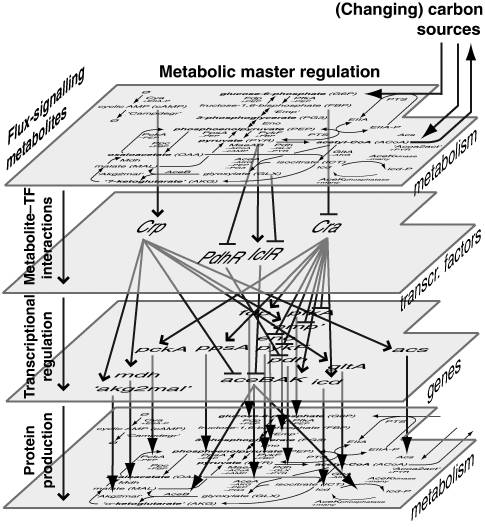
\includegraphics[width=0.4\textwidth]{metabolic_reg}
\caption[Different layers that control the regulation of microbial metabolic operations]
{Different layers that control the regulation of microbial metabolic operations\index{sampling_pseudo}}
\label{fig:mlayers}
\end{figure}
Transcriptional, translational, allosteric, and post-translational regulations ensure that a microbe can respond to diverse extracellular cues through global and local circuits \cite{Chubukov2014}. Knowing how a microbe senses input and dials a response is important for metabolic engineers trying to direct microbial resources and reactions to specific pathways. Metabolic engineers typically aim to dial flux of certain pathways or specific reactions.

To understand the effect of sensors on the network, through literature search, a comprehensive a list of discovered sensors  and their potential effects are enumerated. Additionally, through literature search, current desires of the engineering community, as well as using the database RegulonDB \cite{doi:10.1093/nar/gkv1156} which consists of TFs and their targets, a comprehensive list of dials are enumerated. Data from RegulonDB will give insight into what pathways the sensors affect.

The objective of this project is the prove the following hypothesis:
\textbf{Sensors contain enough information to predict the values of the dials}.\\
Using the M-model, flux states with various nutrient sources (reflecting what the sensors sense) are generated using Markov Chain Monte Carlo sampling methods. In order to determine the relationship between these flux states, statistical modeling methods with sensor values as input and dials as output will be used. 

Representing microbial regulation as a state of sensor and dial values is a new paradigm that can aid in metabolic engineering. Based on the predictions of the learning model, follow-up experiments can be designed to engineer desired dial parameters (phenotypes) through optimal perturbations to the sensors or the regulatory network.

%%%%%%%%%%%%%%%%%%%%%%%%%%%%%%%%%%%%%%%%%%%%%%%%%%%%%%%%%%%

\chapter{Background}

\section{Sensors}
Cells have built-in sensors that can react to certain cues, directly and indirectly. In addition to nutrient sensors, which measure the concentration of nutrients, metabolic flux sensors have recently been discovered \cite{Kochanowski1130}. Flux sensors measure the rate of certain enzymatic reactions, and then adjust, or dial, certain reactions and pathways flux. One example as shown in figure \ref{fig:flux} from \cite{Kochanowski1130} paper is a glycolytic flux sensor represented by fructose -1,6-bisphosphate (FBP), which then represses the transcription factor (TF) Cra, affecting downstream processes. 

\begin{figure}[h] 
\centering
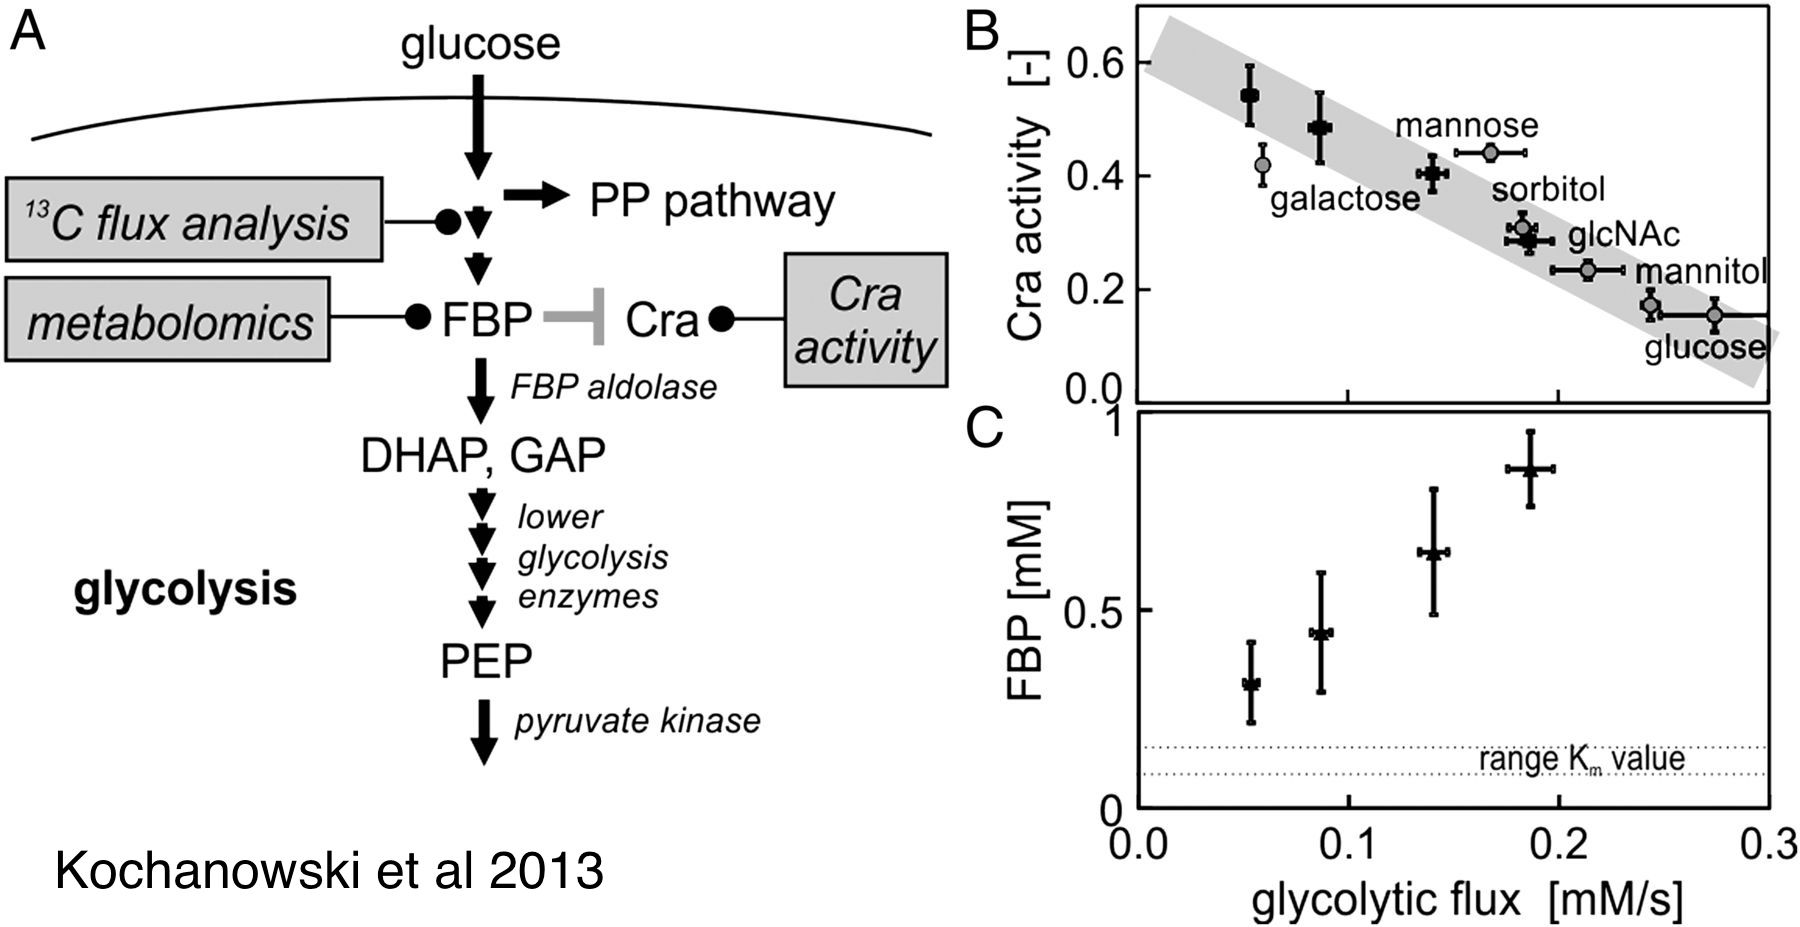
\includegraphics[width=0.6\textwidth]{Flux_sensor}
\caption[Glycolytic flux sensor]
{Glycolytic flux sensor\index{sampling_pseudo}}
\label{fig:flux}
\end{figure}

Table \ref{tab:sensors} provides a list of all the sensors and their respective BiGG \cite{doi:10.1093/nar/gkv1049} IDs. For the purposes of this project, only the first four sensors were chosen i.e only PGI, nadh\textunderscore c, nadhp\textunderscore c and 
EX\textunderscore o2\textunderscore e sensors are used to predict the dial values.

\vspace{0.25in}
\begin{table}[!ht]
\caption[List of sensors and their corresponding BiGG IDs]{List of sensors and their BiGG IDs}

\vspace{-0.25in}
\begin{center}
\begin{tabular}{|p{2in}|p{2.1in}|p{0.75in}|}
\hline
Sensor & BiGG ID  & Literature reference \\

\hline
fructose-1,6-bisphosphatase (FBP) & PGI & \cite{Kochanowski1130}\\

\hline
Aerobic respiration control protein ArcA (ArcA), Fumarate and Nitrate reductase Regulatory (FNR) & nadh\textunderscore c metabolite & \cite{10.1371/journal.pgen.1004264}\\

\hline
Fumarate and Nitrate reductase Regulatory (FNR)& EX\textunderscore o2\textunderscore e & \cite{10.1371/journal.pgen.1004264}\\

\hline
&nadph\textunderscore c metabolite &\\


\hline
Cyclic adenosine monophosphate (cAMP) & ADNCYC & \cite{Chubukov2014}\\

\hline
L-glutamine (gln\textunderscore \textunderscore L\textunderscore c)& EX\textunderscore gln\textunderscore \textunderscore L\textunderscore e; GLNS; GLUDy & \cite{Chubukov2014}\\

\hline

\end{tabular}
\end{center}
\label{tab:sensors}
\end{table}

\section{Dials}
A dial is defined as a change in flux splits between two different pathways. Figure \ref{fig:dial_1} from \cite{Chubukov2014} shows a pictorial representation of dial. One example is dialing flux from glycolysis to pentose-phosphate pathways as shown in figure \ref{fig:dial_2}\\
Table \ref{tab:dials} lists all the dials and the respective BiGG IDs. For the purposes of this project, only the first three dials were chosen i.e only Pentose phosphate vs glycolysis, Fermentation - Pyruvate and Fermentation - Acetyl-CoA dials.

\vspace{0.25in}
\begin{table}[!ht]
\caption[List of sensors and their corresponding BiGG IDs]{List of sensors and their BiGG IDs}

\vspace{-0.25in}
\begin{center}
\begin{tabular}{|p{2in}|p{2.1in}|}
\hline
Dial & BiGG ID\\

\hline
Pentose phosphate vs glycolysis & PGI / G6PDH2r \\

\hline
Fermentation -- Pyruvate & LDH\textunderscore D / PDH, PFL / PDH\\
\hline
Fermentation -- Acetyl-CoA & PTAr / ACALD, PTAr / CS\\

\hline
Glyoxylate shunt & ICL - ICDHyr\\


\hline
Embden-Meyerhoff-Parnass (EMP) vs Entner-Doudoroff (ED) & GND / EDD\\

\hline
Pep Split & (GLCptspp + PYK ) / PPC\\

\hline
NH4 uptake options & GLUDy / GLUSy, GLUDy / GLNS\\

\hline

\end{tabular}
\end{center}
\label{tab:dials}
\end{table}

\begin{figure}[h] 
\centering
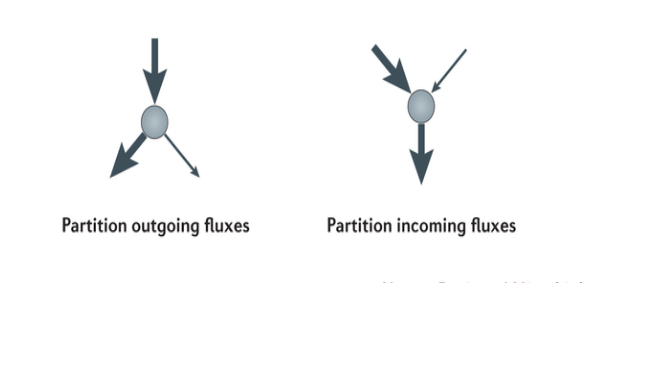
\includegraphics[width=0.4\textwidth]{dial_1}
\caption[Pictographic representation of Dial]
{Pictographic representation of Dial\index{sampling_pseudo}}
\label{fig:dial_1}
\end{figure}

\begin{figure}[h] 
\centering
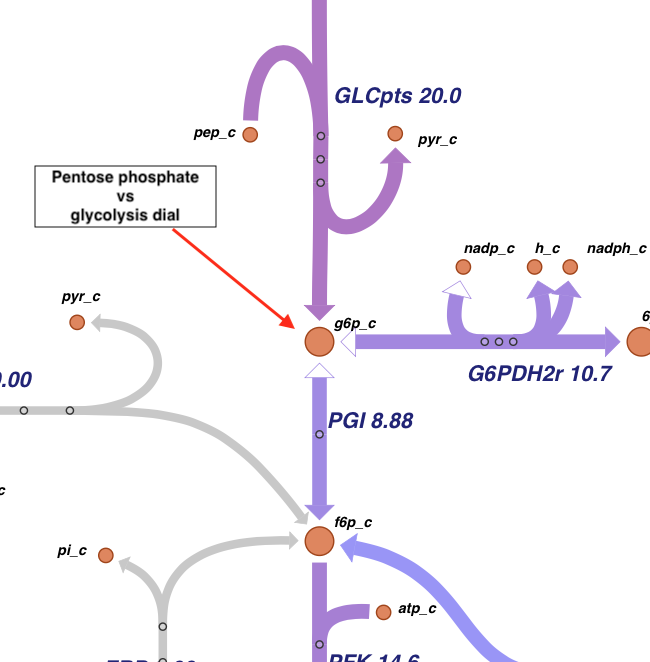
\includegraphics[width=0.4\textwidth]{dial_2}
\caption[Pentose-phosphate vs glycolysis dial]
{Pentose-phosphate vs glycolysis dial\index{sampling_pseudo}}
\label{fig:dial_2}
\end{figure}

\chapter{Related Work}
\textbf{TODO : fill it up}\\

\begin{figure}[!tbp]
  \centering
  \begin{minipage}[b]{0.4\textwidth}
    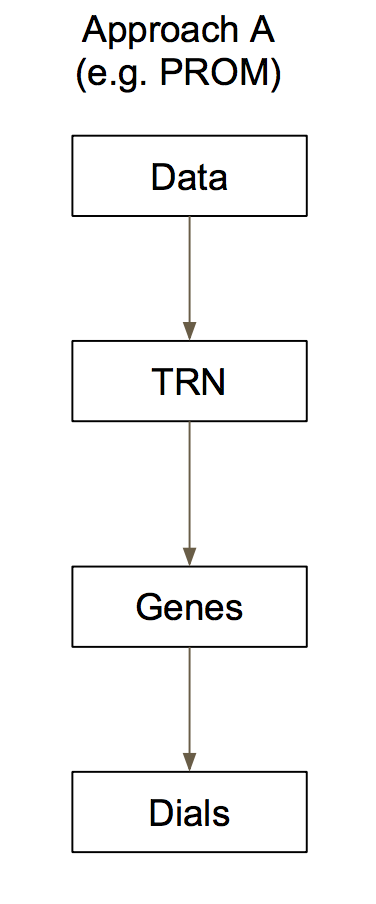
\includegraphics[width=\textwidth]{PROM}
    \caption[System design PROM modeling approach]{System design of PROM modeling approach}
    \label{fig:prom}
  \end{minipage}
  \hfill
  \begin{minipage}[b]{0.4\textwidth}
    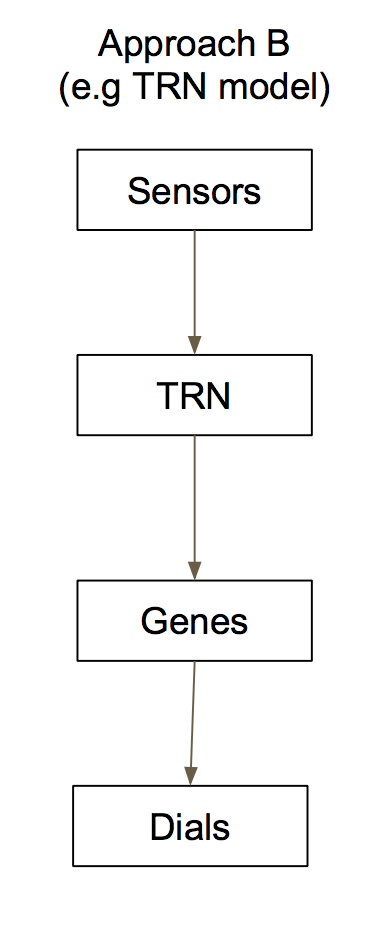
\includegraphics[width=\textwidth]{TRN}
    \caption[System design of TRN modeling approach]{System design of TRN modeling approach}
\label{fig:trn}
  \end{minipage}
\end{figure}

\chapter{System Design}
The block diagram of the system is as show in figure \ref{fig:sys}

\begin{figure}[h] 
\centering
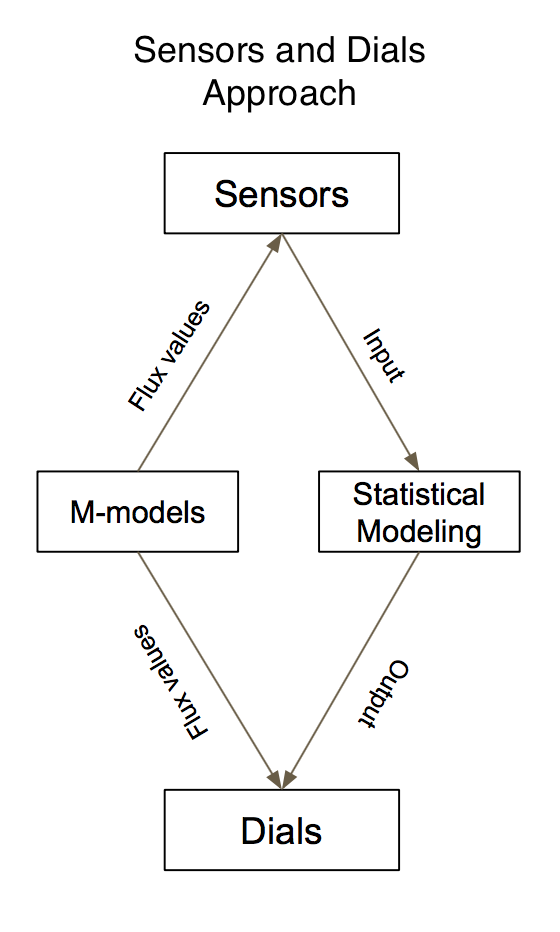
\includegraphics[width=0.4\textwidth]{my_model}
\caption[System design of the sensors and dials modeling approach]
{System design of the sensors and dials modeling approach\index{sampling_pseudo}}
\label{fig:sys}
\end{figure}

\vspace{0.25in}
If the values of the sensors are known, using statistical modeling, the values of the dials can be predicted.\\
This approach is different from both PROM and TRN approaches shown in figures \ref{fig:prom} and \ref{fig:trn}. It does not require information about the underlying transcription factors or the gene data. One can directly predict the dial values using the sensor values through statistical modeling approaches.

The following chapters will detail the dataset used in the modeling task. A number of models with varying accuracy are used to predict the dial values. The workings and the results of each of the models are detailed in chapters \ref{chap:method} and \ref{chap:results}

\chapter{Dataset}

The dataset consists of metabolic flux values of Escherichia coli str. K-12 substr. MG1655 \cite{Blattner1453} obtained by Monte Carlo Markov chain (MCMC) sampling of BiGG \cite{doi:10.1093/nar/gkv1049} models as seen in table \ref{tab:bigg}. 


\vspace{0.25in}
\begin{table}[!ht]
\caption[BiGG models]{List of BiGG models and their reference}

\vspace{-0.25in}
\begin{center}
\begin{tabular}{|p{1in}|p{1in}|}
\hline
BiGG Model  & Reference \\

\hline
iJO1366 & \cite{Orth535} \\

\hline
iML1515 & \cite{Monk2017} \\

\hline

\end{tabular}
\end{center}
\label{tab:bigg}
\end{table}


\vspace{0.25in}
\begin{table}[!ht]
\caption[Sampling conditions]{List of Sampling conditions used in MCMC sampling}

\vspace{-0.25in}
\begin{center}
\begin{tabular}{|p{1.2in}|p{1.4in}|}
\hline
Sources  & Lower bound values\\
\hline
\verb|EX_glc__D_e| & \verb|0, 5 and 10| \\
\hline
\verb|EX_xyl__D_e| &  \verb|0, 5 and 10| \\
\hline
\verb|EX_rib__D_e| &  \verb|0, 5 and 10| \\
\hline
\verb|EX_glyc_e| &  \verb|0, 5 and 10| \\
\hline
\verb|EX_ac_e| &  \verb|0, 5 and 10| \\
\hline
\verb|EX_pyr_e| &  \verb|0, 5 and 10| \\
\hline
\verb|EX_nh4_e| &  \verb|0 and 1000| \\
\hline
\verb|EX_o2_e| &  \verb|0, 2 and 20| \\
\hline
\verb|EX_arg__L_e| &  \verb|0, 5 and 10| \\
\hline
\verb|EX_asp__L_e| &  \verb|0, 5 and 10| \\
\hline
\verb|EX_ser__L_e| &  \verb|0, 5 and 10| \\
\hline
\verb|EX_cys__L_e| &  \verb|0, 5 and 10| \\
\hline
\verb|EX_pro__L_e| &  \verb|0, 5 and 10| \\
\hline
\verb|EX_ala__L_e| &  \verb|0, 5 and 10| \\
\hline
\verb|EX_trp__L_e| &  \verb|0, 5 and 10| \\
\hline

\end{tabular}
\end{center}
\label{tab:sampling}
\end{table}

\section{Sampling Conditions}
The dataset was created by constraining the MCMC sampling of BiGG models by a set of conditions. The conditions were created by varying the magnitude and direction (positive or negative) of the lower bound values of different Carbon, Nitrogen, Oxygen and Amino acid sources. The complete list of sources is as shown in table \ref{tab:sampling}.  

\section{MCMC Sampling Procedure}
Since the dataset consists of metabolic flux values, the most widely used technique to analyze these fluxes in large-scale metabolic reconstructions is flux balance analysis (FBA). In FBA, a liner objective function , typically the biomass or some biological proxy of it is introduced, and the problem reduces to finding the subspace of the polytope, which optimizes the objective function. If this subspace consists in only one point, the problem can be efficiently solved using linear programming. However, if one is interested in describing more general growth conditions, or is interested in other fluxes than the biomass, different computational strategies must be envisaged. 

As long as no prior knowledge is considered, each point of the polytope is an equally viable metabolic phenotype of the biological system under investigation. Therefore, being able to sample high-dimensional polytopes becomes a theoretical problem with concrete practical applications. From a theoretical standpoint, the problem is known to be NP-hard and thus an approximate solution to the problem must be sought. The approximate solution can be obtained using MCMC sampling technique. MCMC sampling, basically, consists of iteratively collecting samples by choosing random directions from a starting point belonging to the polytope.

For this project, the COBRApy \cite{Ebrahim2013} software was used to perform MCMC sampling. A set of 34 conditions were created using all combinations of sources and lower bound values mentioned in table \ref{tab:sampling}. An example of the sampling condition set is as shown in listing \ref{lst:sample_conds}. The feasibility of each of the samples was checked by running FBA. If the solution objective of FBA (in this case the growth rate) is greater than $0.05$, the optimized model was used for sampling. Before MCMC sampling was run, the lower bound value of the biomass function was set to $99\%$ of the solution objective obtained after performing FBA. For each feasible condition, a sample of $1000$ was collected. The dataset consisted of $340000$ datapoints.

\lstset{
string=[s]{"}{"},
stringstyle=\color{blue},
comment=[l]{:},
commentstyle=\color{black},
}
\begin{spacing}{1}
\begin{lstlisting}[caption={Sampling conditions}, label={lst:sample_conds}]
[
{
    "EX_nh4_e": -1000,
    "EX_o2_e": 0,
    "EX_glc__D_e": -10
},
{
    "EX_xyl__D_e": -10,
    "EX_nh4_e": -1000,
    "EX_o2_e": 0
},
{
    "EX_arg__L_e": -10,
    "EX_nh4_e": -1000,
    "EX_o2_e": 0,
    "EX_glc__D_e": -10
},
{
    "EX_ser__L_e": -10,
    "EX_nh4_e": -1000,
    "EX_o2_e": -20,
    "EX_glc__D_e": -10
}

]
\end{lstlisting}
\end{spacing}

The COBRApy software contains implementation of two different types of sampling techniques namely optGpSampler \cite{10.1371/journal.pone.0086587} and ACHR Sampler \cite{Thiele25032005}. From literature and from extensive experimentation as shown in \href{https://github.com/cdiener/cobra-docker/blob/master/sampling_benchmark.ipynb}{Cobrapy sampling benchmarking} website, it was discovered that ACHR sampler performed better than optGpSampler. For the purposes of this project, ACHR sampler was used to perform sampling.\\
The pseudocode of the sampling technique used is as shown in fig \ref{fig:sampling_pseudo}

\begin{figure}[h] 
\centering
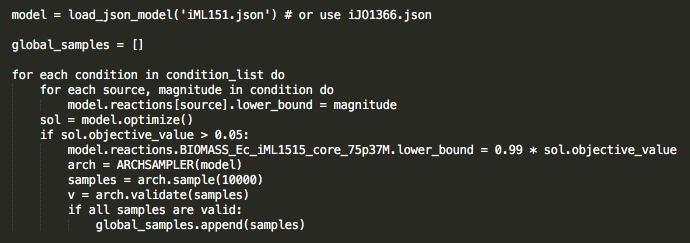
\includegraphics[width=0.5\textwidth]{sampling_pseudo}
\caption[Sampling pseudocode]
{Pseudocode of the sampling technique\index{sampling_pseudo}}
\label{fig:sampling_pseudo}
\end{figure}


\section{Dataset Validation}
In order to validate the samples obtained using MCMC sampling, a number of experiments were conducted and they are enumerated below.
\subsection{Validate function}
The most readily available validation technique is the "validate" function that's part of the ARCH sampler library. The validate function checks to see if the set of points are feasible and give detailed information about feasibility violations. 

\subsection{Auto-correlation Plots}
The second technique used to validate the samples is by drawing autocorrelation plot. From the fig \ref{fig:acp} we can see that the autocorrelation tends to be close to 0 towards the end of the series. The sampling experiment was run repeatedly to select the best dataset with the lowest autocorrelation value.

\begin{figure}[h] 
\centering
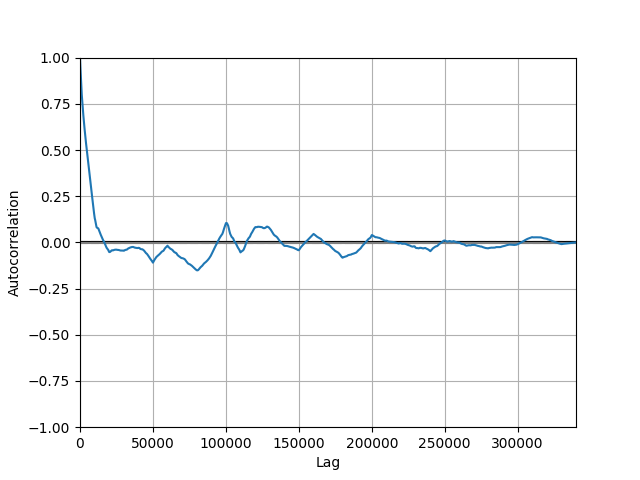
\includegraphics[width=0.5\textwidth]{acp_330k}
\caption[Autocorrelation plot]
{Autocorrelation plot for the 340k flux data\index{acp}}
\label{fig:acp}
\end{figure}

\subsection{Drawing Pathway Maps in Escher}
The third technique used to validate the samples is by drawing pathway maps in Escher \cite{10.1371/journal.pcbi.1004321}. This will rule out the obvious errors in the sampling data like loops that are out of the ordinary. 

\subsection{Gelman and Rubin Test}
The fouth technique used to validate the samples is using the Gelman and Rubin test as explained in \cite{10.1371/journal.pone.0086587} under the Empirical Convergence Diagnostics section. The R value obtained was $1.032$. This indicated that the dataset has achieved empirical convergence. 

\chapter{Methodology}\label{chap:method}
In order to test the hypothesis about correlation between sensors and dials,
initial set of line plots of each sensor and dial were drawn. Once a correlation was indeed noticed, statistical modeling was done on the data. A number of statistical modeling techniques like liner regression, tree based models and ensemble learning models were used 

\section{Initial Analysis} \label{sec:initial Analysis}
A line plot consisting of both sensor and dial values were plotted. Since the dataset consisted of $340000$ datapoints, binned scatter plots of sensor vs dial were drawn. \\
A high correlation was noticed in case of PGI sensor and PGI-G6PDH2r dial which can be seen in fig \ref{fig:binned}. Similar correlation can be seen in figures \ref{fig:o2ldhline}, \ref{fig:nadhline} and \ref{fig:o2pgiline}

%\vspace{-0.25in}
\begin{figure}[h] 
\centering
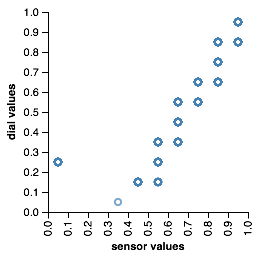
\includegraphics[width=0.5\textwidth]{PGI_sensor_PGI_G6PDH2r}
\caption[Binned scatter plot of PGI sensor vs PGI-G6PDH2r dial]
{A binned scatter plot of PGI sensor vs PGI-G6PDH2r dial.\index{binned scatter}}
\label{fig:binned}
\end{figure}

%\vspace{-0.25in}
\begin{figure}[h] 
\centering
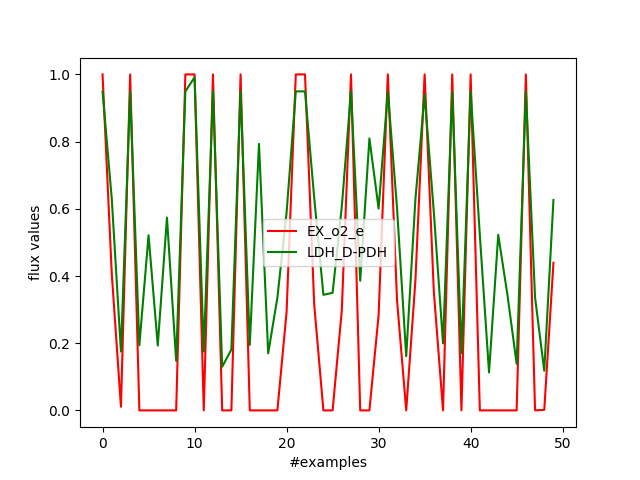
\includegraphics[width=0.5\textwidth]{EX_o2_e_LDH_D_PDH_lineplot_50}
\caption[EX\textunderscore o2 \textunderscore c with LDH \textunderscore D - PDH line plot]
{A line plot of Oxygen exchange reaction and $(LDH_D, PDH)$  dial.\index{o2Ldh-Pdh line plot}}
\label{fig:o2ldhline}
\end{figure}

%\vspace{-0.25in}
\begin{figure}[h] 
\centering
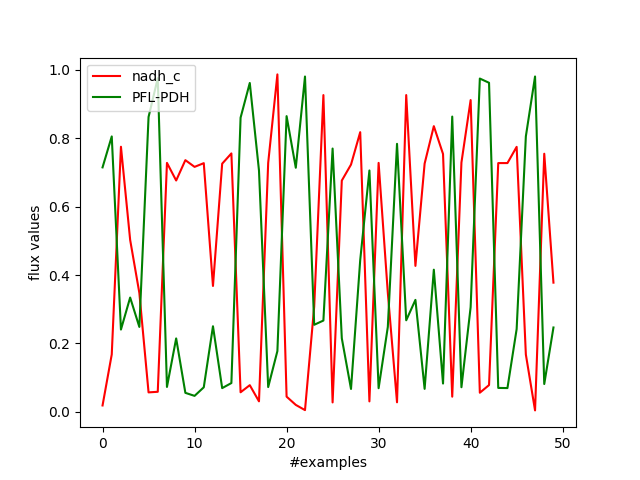
\includegraphics[width=0.5\textwidth]{nadh_c_PFL_PDH_lineplot_50}
\caption[nadh \textunderscore c with PFL-PDH line plot]
{A line plot of nadh\textunderscore c and $(PFL-PDH)$ dial.\index{nadhPFL-PDH line plot}}
\label{fig:nadhline}
\end{figure}

%\vspace{-0.25in}
\begin{figure}[h] 
\centering
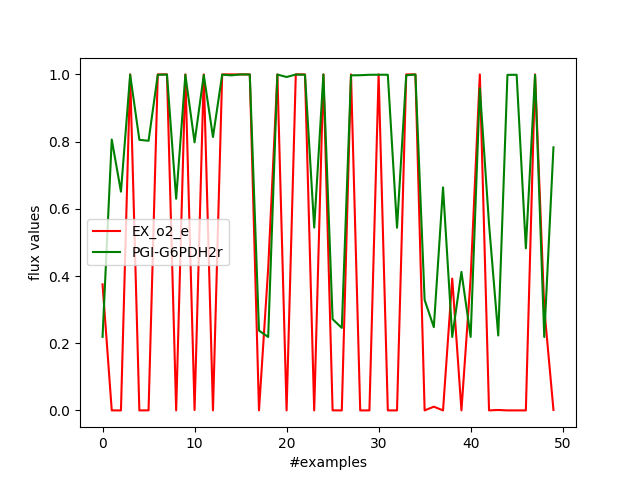
\includegraphics[width=0.5\textwidth]{EX_o2_e_PGI_G6PDH2r_lineplot_50}
\caption[EX\textunderscore o2 \textunderscore c with PGI-G6PDH2r line plot]
{A line plot of EX\textunderscore o2 \textunderscore c PGI-G6PDH2r dial.\index{o2Pgi-G6pdh2r}}
\label{fig:o2pgiline}
\end{figure}

\section{Inputs and Outputs}
The inputs and outputs are flux values of the corresponding sensors and dials.\\ Since the flux values varies from $-1000$ to $+1000$, a number of normalization techniques namely atan, log and \textbf{min-max} were used. After careful redrawing of line plots mentioned in section \ref{sec:initial Analysis}, it was established that min-max normalization best suited the data.\\
The dials are a pair of metabolic reactions. Different methods namely ratio of the dial and \textbf{difference between the absolute values of the dials}, were used to represent the dials. The absolute value of the dials were taken into consideration to prevent penalization while calculating the difference. After careful redrawing of line plots mentioned in section \ref{sec:initial Analysis}, it was established that difference between the absolute values of the dials best suited the data.\\

The dataset was split into training-validation-testing sets. The split was 70\%-10\%-20\% respectively. The dataset was shuffled to make sure that all the conditions were seen in all the sets. \\
A seperate model was built for each dials. 

\section{Statistical Modeling}
    Statistical modeling was done using Scikit-learn \cite{scikit-learn}, \cite{sklearn_api} library.
\subsection{Linear Regression}
The line plots in figures \ref{fig:binned}, \ref{fig:o2ldhline}, \ref{fig:nadhline} and \ref{fig:o2pgiline}, it can be seen that there exist a liner correlation between each of the sensors and dials. Since a linear correlation exists, the statistical model best suited was liner regression. The results for linear regression are as shown in section \ref{sec:lr}

\subsection{Extreme Gradient Boosted Trees}\label{sec:xgboost}
From section \ref{sec:lr}, it is seen that linear regression doesn't perform as well as one would expect. Although there exists a linear relationship between each of the sensors and the dials, a combination of all the sensors leads to non-linearity. Since linear regression tries to fit a straight line for the dataset at hand, it fails to capture this non-linearity. In order to learn this non-linearity, ensemble learning techniques were employed.\\
Extreme Gradient Boosted Trees \string(XGBoost) \cite{Chen:2016:XST:2939672.2939785} is a class of gradient boosted tree algorithm that employs the tree ensemble model.\\
The XGBoost library has in-built APIs to retrieve feature importance. Feature importance provides a score that indicates how useful or valuable each feature is in the construction of the boosted decision trees within the model. The more an attribute is used to make key decisions with decision trees, the higher its relative importance.\\
This importance is calculated explicitly for each attribute in the dataset, allowing attributes to be ranked and compared to each other. Importance is calculated for a single decision tree by the amount that each attribute split point improves the performance measure, weighted by the number of observations the node is responsible for. The performance measure may be the purity (Gini index) used to select the split points or another more specific error function. The feature importances are then averaged across all of the the decision trees within the model.\\
Feature importance is calculated as follows -
\begin{verbatim}
feature_imp = [0] * n_features
#traverse tree
for each internal_node that splits on feature i
    err = compute(error reduction of that node)
    feature_imp[i] = feature_imp[i] + err * len(samples through internal_node)
\end{verbatim}
The results from XGBoost and the feature importance plots are as shown in section \ref{sec:xgboostRes}\\
\textbf{TODO: Add biological significance}

\subsection{Decision Tree Regressor}
From section \ref{sec:xgboostRes}, we can see that although XGBoost performs better than linear regression, it is still not up to the mark. This is clearly visible in figure \ref{fig:PtarAcaldXgb}. We see that a large number of points deviate from the \ang{45} line i.e from the actual value. This is because XGBoost, which employs boosting technique, is based on weak learners \string(high bias, low variance).\\
In terms of decision trees, weak learners are shallow trees, sometimes even as small as decision stumps (trees with two leaves). Boosting reduces error mainly by reducing bias and also to some extent variance, by aggregating the output from many models. The idea is to add a classifier/regressor at a time, so that the next classifier/regressor is trained to improve the already trained ensemble.\\
With respect to this dataset, XGBoost overfits to the training data and hence results in lower accuracy. On the other hand, decision trees by means of not employing weak learners, does not overfit the data and hence leads to more accurate result. XGBoost also requires a lot of parameter tuning and either the lack of tuning or extensive tuning can lead to overfitting.\\
The feature importance calculation is done similarly as in section \ref{sec:xgboost}\\ The results from decision tree regressor and feature importance plots are as shown in section \ref{sec:dtrRes}


\subsection{Random Forest Regressor}
From section \ref{sec:dtrRes}, we can see that random forest regressor performs marginally better than decision trees.
Random Forest creates a large number of decision trees based on bagging. The basic idea is to resample the data over and over and for each sample train a new classifier/regressor. Different classifiers/regressors overfit the data in a different way, and through voting those differences are averaged out.\\
The feature importance calculation is done similarly as in section \ref{sec:xgboost}\\
The results from random forest regressor and feature importance plots are as shown in section \ref{sec:rfrRes}


%%%%%%%%%%%%%%%%%%%%%%%%%%%%%%%%%%%%%%%%%%%%%%%%%%%%%%%%%%%%%%%%%%%%%%%%%%%%%%%%%%%

\chapter{Results} \label{chap:results}
The results of statistical modeling will be reported in terms of mean-squared-error \string(MSE), Pearson-r and Coefficient $R\string^2$ values. The results will be accompanied by scatter plots of actual vs predicted values.

\section{Linear Regression} \label{sec:lr}
Table \ref{tab:lr} reflects the results from linear regression.\\
From figures \ref{fig:PgiG6pdh2rLr}, \ref{fig:PtarCsLr}, \ref{fig:PflPdhLr}, \ref{fig:LdhPdhLr} and \ref{fig:PtarAcaldLr}, we can see that even though there exists a liner correlation between each sensor and dials, when all the sensors are considered together, the model performs poorly. 

\vspace{0.25in}
\begin{table}[!ht]
\caption[Linear regression results]{Results from Linear Regression}

\vspace{-0.25in}
\begin{center}
\begin{tabular}{|p{1.3in}|p{1in}|p{1in}|p{1.1in}|}
\hline
Dial & MSE  & Pearson-r & Coefficient R\string^2 \\

\hline
\string(PGI, G6PDH2r) & 0.0100 & 0.9554 & 0.9128 \\

\hline
\string(LDH\textunderscore D, PDH) & 0.0143 & 0.9297 & 0.8639\\

\hline
\string(PFL, PDH) & 0.0113 & 0.9491 & 0.8639\\

\hline
\string(PTAr, ACALD) &  0.0246 & 0.8339 & 0.6932\\

\hline
\string(PTAr, CS) & 0.0290 & 0.8343 & 0.6921\\

\hline

\end{tabular}
\end{center}
\label{tab:lr}
\end{table}

%\vspace{-0.25in}
\begin{figure}[h] 
\centering
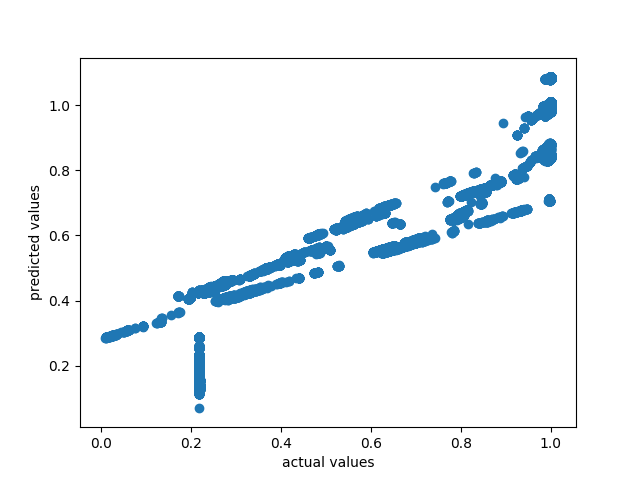
\includegraphics[width=0.5\textwidth]{PGI_G6PDH2r_lr.png}
\caption[Linear Regression scatter plot of actual vs predict values for $(PGI, G6PDH2r)$ dial]
{Linear Regression scatter plot of actual vs predict values for $(PGI, G6PDH2r)$ dial\index{Linear Regression scatter plot for $(PGI, G6PDH2r)$ dial}}
\label{fig:PgiG6pdh2rLr}
\end{figure}

%\vspace{-0.25in}
\begin{figure}[h] 
\centering
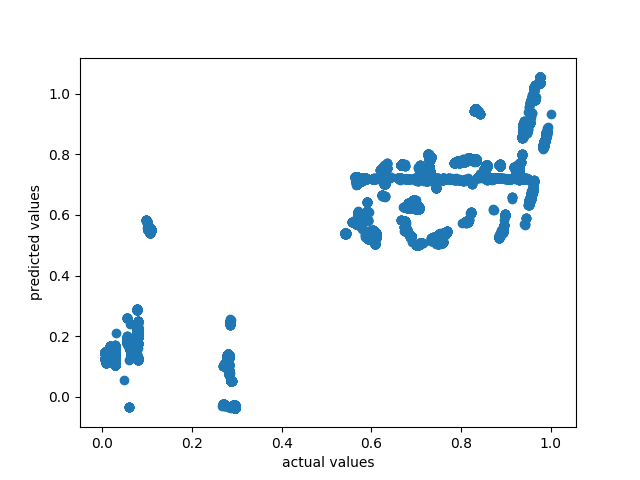
\includegraphics[width=0.5\textwidth]{PTAr_CS_lr}
\caption[Linear Regression scatter plot of actual vs predict values for $(PTAr, CS)$ dial]
{Linear Regression scatter plot of actual vs predict values for $(PTAr, CS)$ dial\index{Linear Regression scatter plot for $(PTAr, CS)$ dial}}
\label{fig:PtarCsLr}
\end{figure}

%\vspace{-0.25in}
\begin{figure}[h] 
\centering
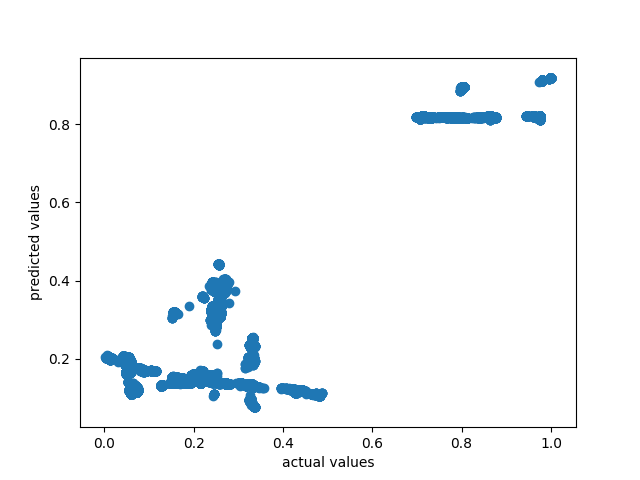
\includegraphics[width=0.5\textwidth]{PFL_PDH_lr}
\caption[Linear Regression scatter plot of actual vs predict values for $(PFL, PDH)$ dial]
{Linear Regression scatter plot of actual vs predict values for $(PFL, PDH)$ dial\index{Linear Regression scatter plot for $(PFL, PDH)$ dial}}
\label{fig:PflPdhLr}
\end{figure}

%\vspace{-0.25in}
\begin{figure}[h] 
\centering
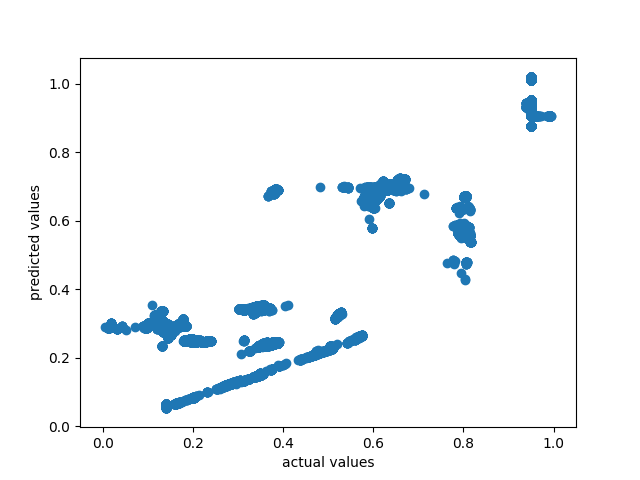
\includegraphics[width=0.5\textwidth]{LDH_D_PDH_lr}
\caption[Linear Regression scatter plot of actual vs predict values for \string(LDH\textunderscore D, PDH) dial]
{Linear Regression scatter plot of actual vs predict values for \string(LDH\textunderscore D, PDH) dial\index{Linear Regression scatter plot for \string(LDH\textunderscore D, PDH) dial}}
\label{fig:LdhPdhLr}
\end{figure}

%\vspace{-0.25in}
\begin{figure}[h] 
\centering
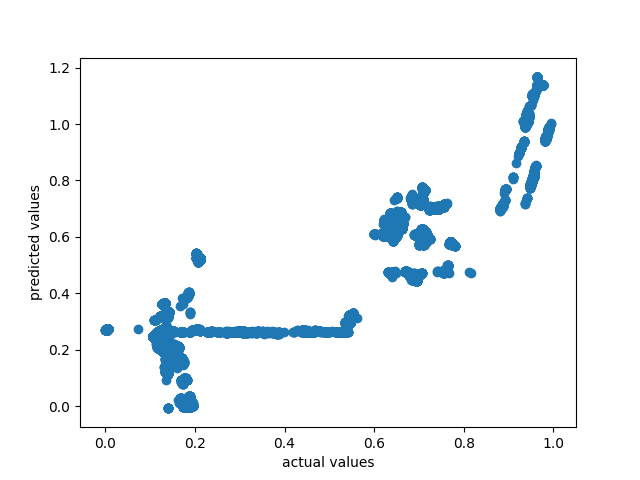
\includegraphics[width=0.5\textwidth]{PTAr_ACALD_lr}
\caption[Linear Regression scatter plot of actual vs predict values for $(PTAr, ACALD)$ dial]
{Linear Regression scatter plot of actual vs predict values for $(PTAr, ACALD)$ dial\index{Linear Regression scatter plot for $(PTAr, ACALD)$ dial}}
\label{fig:PtarAcaldLr}
\end{figure}

%%%%%%%%%%%%%%%%%%%%%%%%%%%%%%%%%%%%%%%%%%%%%%%%%%%%%%%%%%%%%%%%%%%%%%%%%%%%%%%%%%%

\section{Extreme Gradient Boosted Trees} \label{sec:xgboostRes}

Table \ref{tab:Xgboost} reflects the results from XGBoost regressor.
From figures \ref{fig:PgiG6pdh2rXgb}, \ref{fig:PtarCsXgb}, \ref{fig:PflPdhXgb}, \ref{fig:LdhPdhXgb} and \ref{fig:PtarAcaldXgb}, we can see that the xgboost regressor performs better than linear regression. 
Figures \ref{fig:PgiG6pdh2rXgbImp}, \ref{fig:PtarCsXgbImp}, \ref{fig:PflPdhXgbImp}, \ref{fig:LdhPdhXgbImp} and \ref{fig:PtarAcaldXgbImp} shows the feature importance plots for each of the dials.\\
\vspace{0.25in}
\begin{table}[!ht]
\caption[XGBoost Regressor results]{Results from XGBoost Regressor}

\vspace{-0.25in}
\begin{center}
\begin{tabular}{|p{1.3in}|p{1in}|p{1in}|p{1.1in}|}
\hline
Dial & MSE  & Pearson-r & Coefficient R\string^2 \\

\hline
\string(PGI, G6PDH2r) & 0.000247 & 0.99929 & 0.997847 \\

\hline
\string(LDH\textunderscore D, PDH) & 0.000609 & 0.997753 & 0.994214\\

\hline
\string(PFL, PDH) & 0.000744 & 0.997318 & 0.993482\\

\hline
\string(PTAr, ACALD) & 0.001241 & 0.994060 & 0.9845706\\

\hline
\string(PTAr, CS) & 0.001215 & 0.995115 & 0.9873441\\

\hline

\end{tabular}
\end{center}
\label{tab:Xgboost}
\end{table}

%\vspace{-0.25in}
\begin{figure}[h] 
\centering
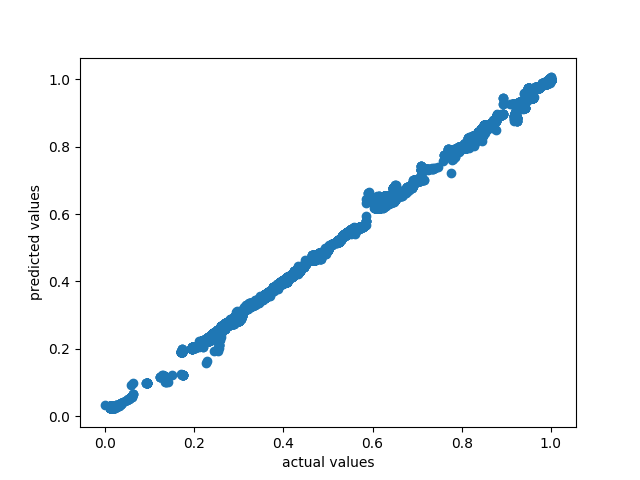
\includegraphics[width=0.5\textwidth]{PGI_G6PDH2r_xgboost_no_params}
\caption[XGBoost Regressor scatter plot of actual vs predict values for $(PGI, G6PDH2r)$ dial]
{XGBoost Regressor scatter plot of actual vs predict values for $(PGI, G6PDH2r)$ dial\index{XGBoost Regressor scatter plot for $(PGI, G6PDH2r)$ dial}}
\label{fig:PgiG6pdh2rXgb}
\end{figure}

%\vspace{-0.25in}
\begin{figure}[h] 
\centering
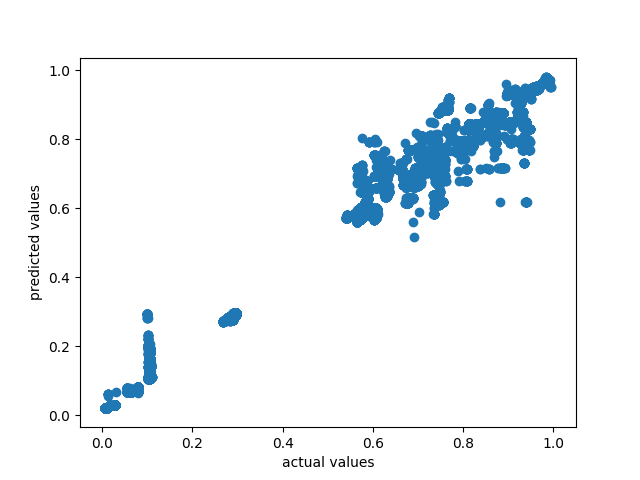
\includegraphics[width=0.5\textwidth]{PTAr_CS_xgboost_no_params}
\caption[XGBoost Regressor scatter plot of actual vs predict values for $(PTAr, CS)$ dial]
{XGBoost Regressor scatter plot of actual vs predict values for $(PTAr, CS)$ dial\index{XGBoost Regressor scatter plot for $(PTAr, CS)$ dial}}
\label{fig:PtarCsXgb}
\end{figure}

%\vspace{-0.25in}
\begin{figure}[h] 
\centering
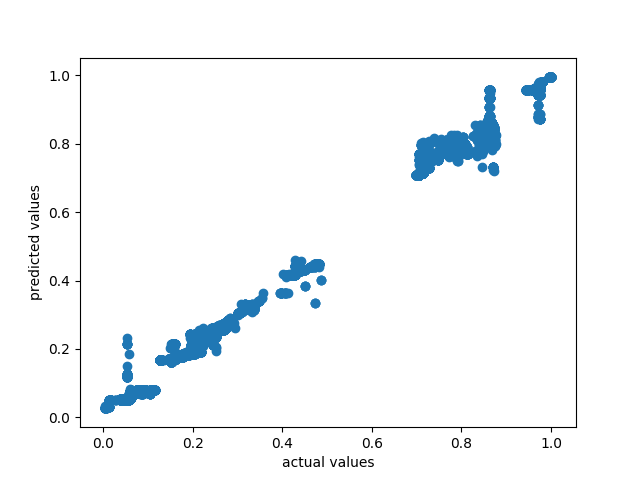
\includegraphics[width=0.5\textwidth]{PFL_PDH_xgboost_no_params}
\caption[XGBoost Regressor scatter plot of actual vs predict values for $(PFL, PDH)$ dial]
{XGBoost Regressor scatter plot of actual vs predict values for $(PFL, PDH)$ dial\index{XGBoost Regressor scatter plot for $(PFL, PDH)$ dial}}
\label{fig:PflPdhXgb}
\end{figure}

%\vspace{-0.25in}
\begin{figure}[h] 
\centering
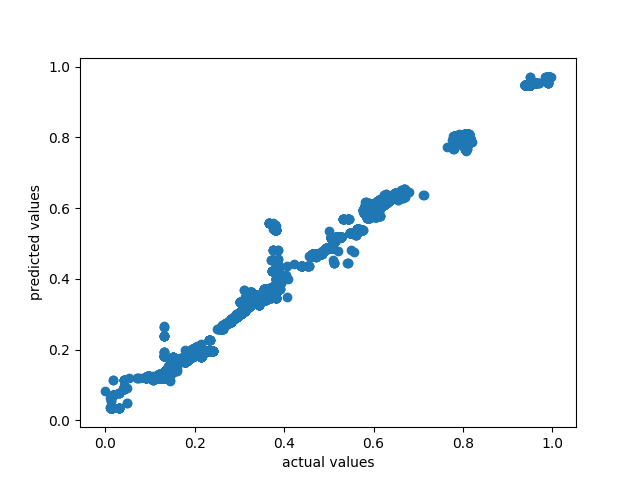
\includegraphics[width=0.5\textwidth]{LDH_D_PDH_xgboost_no_params}
\caption[XGBoost scatter plot of actual vs predict values for \string(LDH\textunderscore D, PDH) dial]
{XGBoost Regressor scatter plot of actual vs predict values for $(LDH_D, PDH)$ dial\index{XGBoost Regressor scatter plot for \string(LDH\textunderscore D, PDH) dial}}
\label{fig:LdhPdhXgb}
\end{figure}

%\vspace{-0.25in}
\begin{figure}[h] 
\centering
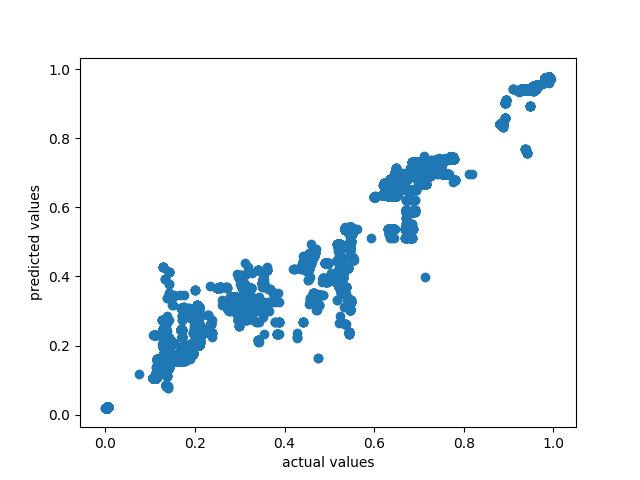
\includegraphics[width=0.5\textwidth]{PTAr_ACALD_xgboost_no_params}
\caption[XGBoost Regressor scatter plot of actual vs predict values for $(PTAr, ACALD)$ dial]
{XGBoost Regressor scatter plot of actual vs predict values for $(PTAr, ACALD)$ dial\index{XGBoost Regressor scatter plot for $(PTAr, ACALD)$ dial}}
\label{fig:PtarAcaldXgb}
\end{figure}

%\vspace{-0.25in}
\begin{figure}[h] 
\centering
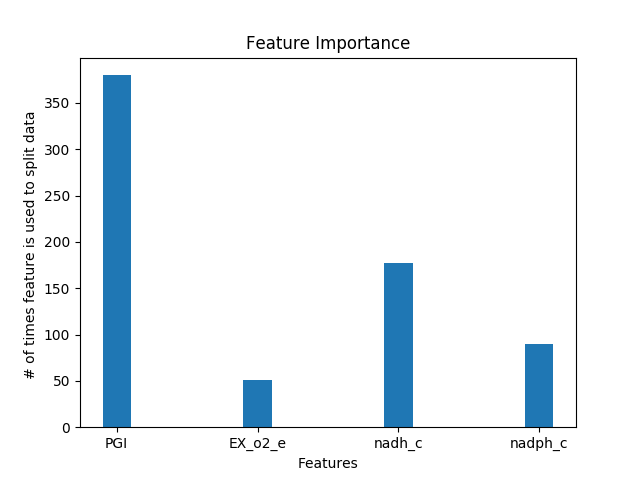
\includegraphics[width=0.5\textwidth]{PGI_G6PDH2r_xgboost_no_params_important_features}
\caption[XGBoost feature importance plot for $(PGI, G6PDH2r)$ dial]
{XGBoost feature importance plot for $(PGI, G6PDH2r)$ dial\index{Feature importance plot for $(PGI, G6PDH2r)$ dial}}
\label{fig:PgiG6pdh2rXgbImp}
\end{figure}

%\vspace{-0.25in}
\begin{figure}[h] 
\centering
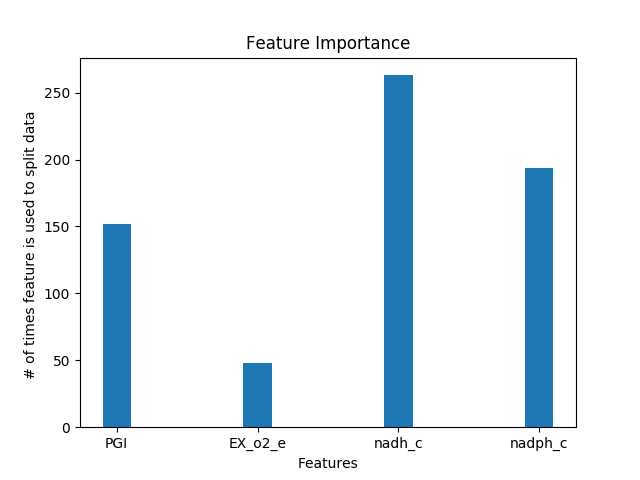
\includegraphics[width=0.5\textwidth]{PTAr_CS_xgboost_no_params_important_features}
\caption[XGBoost feature importance plot for $(PTAr, CS)$ dial]
{XGBoost feature importance plot for $(PTAr, CS)$ dial\index{Feature importance plot for $(PTAr, CS)$ dial}}
\label{fig:PtarCsXgbImp}
\end{figure}

%\vspace{-0.25in}
\begin{figure}[h] 
\centering
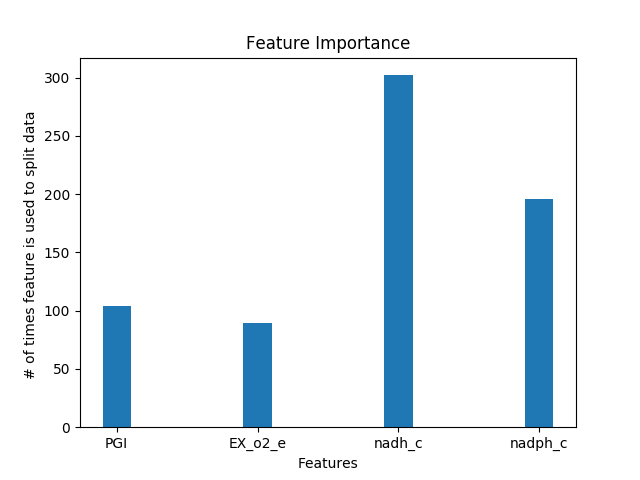
\includegraphics[width=0.5\textwidth]{PFL_PDH_xgboost_no_params_important_features}
\caption[XGBoost feature importance plot for $(PFL, PDH)$ dial]
{XGBoost feature importance plot for $(PFL, PDH)$ dial\index{Feature importance plot for $(PFL, PDH)$ dial}}
\label{fig:PflPdhXgbImp}
\end{figure}

%\vspace{-0.25in}
\begin{figure}[h] 
\centering
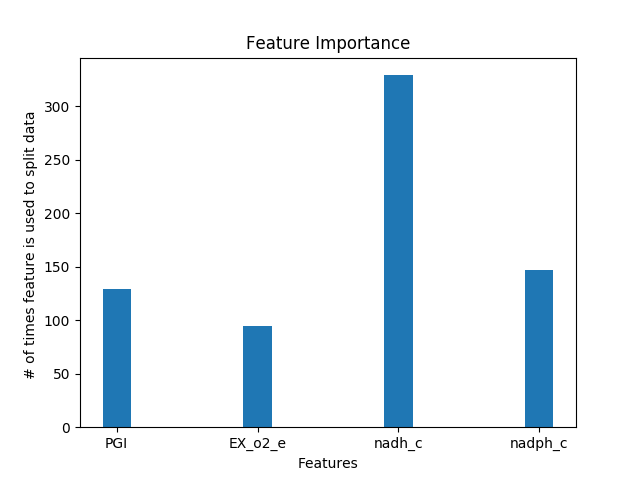
\includegraphics[width=0.5\textwidth]{LDH_D_PDH_xgboost_no_params_important_features}
\caption[XGBoost feature importance plot for \string(LDH\textunderscore D, PDH) dial]
{XGBoost feature importance plot for \string(LDH\textunderscore D, PDH) dial\index{Feature importance plot for \string(LDH\textunderscore D, PDH) dial}}
\label{fig:LdhPdhXgbImp}
\end{figure}

%\vspace{-0.25in}
\begin{figure}[h] 
\centering
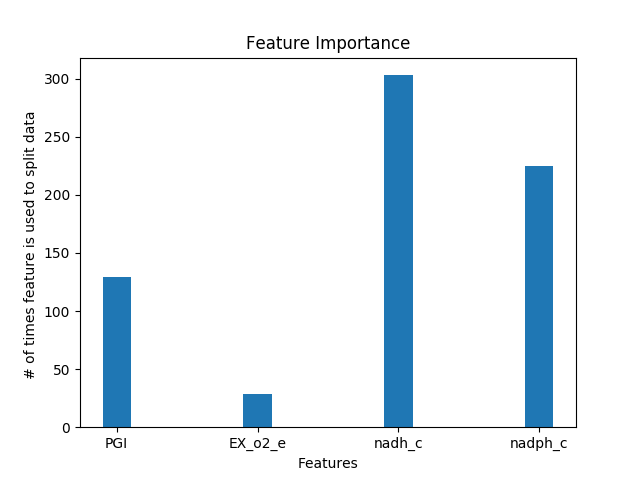
\includegraphics[width=0.5\textwidth]{PTAr_ACALD_xgboost_no_params_important_features}
\caption[XGBoost feature importance plot for $(PTAr, ACALD)$ dial]
{XGBoost feature importance plot for $(PTAr, ACALD)$ dial\index{Feature importance plot for $(PTAr, ACALD)$ dial}}
\label{fig:PtarAcaldXgbImp}
\end{figure}

%%%%%%%%%%%%%%%%%%%%%%%%%%%%%%%%%%%%%%%%%%%%%%%%%%%%%%%%%%%%%%%%%%%%%%%%%%%%%%%%%%%

\section{Decision Tree Regressor}\label{sec:dtrRes}
Table \ref{tab:dtr} reflects the results from decision tree regressor.\\
From figures \ref{fig:PgiG6pdh2rDtr}, \ref{fig:PtarCsDtr}, \ref{fig:PflPdhDtr}, \ref{fig:LdhPdhDtr} and \ref{fig:PtarAcaldDtr}, we can see that the decision tree regressor performs better than xgboost regressor. It's the closest to the actual value with precision up to 5 decimal places.

\vspace{0.25in}
\begin{table}[!ht]
\caption[Decision Tree Regressor results]{Results from Decision Tree Regressor}

\vspace{-0.25in}
\begin{center}
\begin{tabular}{|p{1.3in}|p{1in}|p{1in}|p{1.1in}|}
\hline
Dial & MSE  & Pearson-r & Coefficient R\string^2 \\

\hline
\string(PGI, G6PDH2r) & 2.0987e-06 & 0.99999 & 0.99998 \\

\hline
\string(LDH\textunderscore D, PDH) & 4.9845e-06 & 0.99997 & 0.99995\\

\hline
\string(PFL, PDH) & 1.8038e-06 & 0.99999 & 0.99998\\

\hline
\string(PTAr, ACALD) &  1.75e-05 & 0.99989 & 0.99978\\

\hline
\string(PTAr, CS) & 1.3527e-05 & 0.99992 & 0.99985\\

\hline

\end{tabular}
\end{center}
\label{tab:dtr}
\end{table}


%\vspace{-0.25in}
\begin{figure}[h] 
\centering
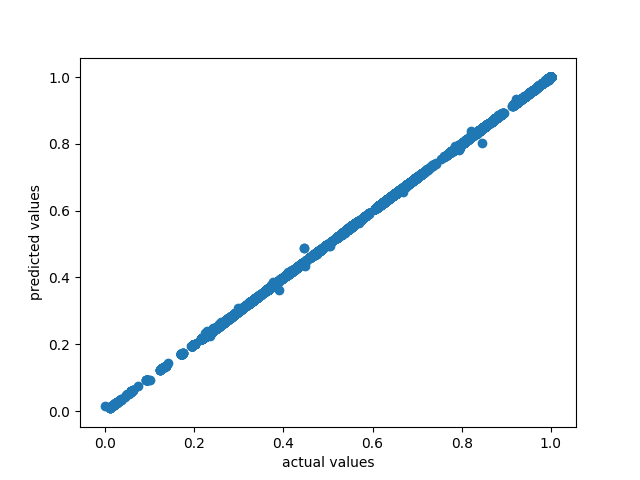
\includegraphics[width=0.5\textwidth]{PGI_G6PDH2r_dtr}
\caption[Decision Tree Regressor scatter plot of actual vs predict values for $(PGI, G6PDH2r)$ dial]
{Decision Tree Regressor scatter plot of actual vs predict values for $(PGI, G6PDH2r)$ dial\index{Decision Tree Regressor scatter plot for $(PGI, G6PDH2r)$ dial}}
\label{fig:PgiG6pdh2rDtr}
\end{figure}

%\vspace{-0.25in}
\begin{figure}[h] 
\centering
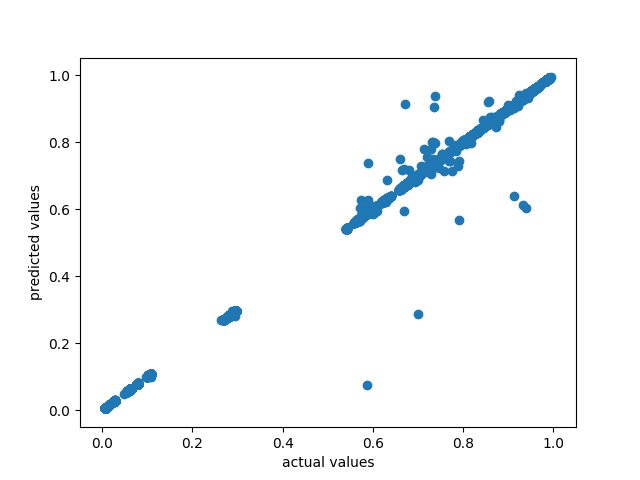
\includegraphics[width=0.5\textwidth]{PTAr_CS_dtr}
\caption[Decision Tree Regressor scatter plot of actual vs predict values for $(PTAr, CS)$ dial]
{Decision Tree Regressor scatter plot of actual vs predict values for $(PTAr, CS)$ dial\index{Decision Tree Regressor scatter plot for $(PTAr, CS)$ dial}}
\label{fig:PtarCsDtr}
\end{figure}

%\vspace{-0.25in}
\begin{figure}[h] 
\centering
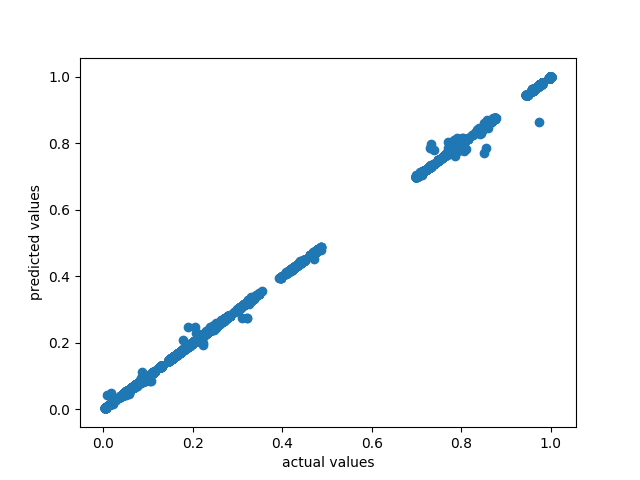
\includegraphics[width=0.5\textwidth]{PFL_PDH_dtr}
\caption[Decision Tree Regressor scatter plot of actual vs predict values for $(PFL, PDH)$ dial]
{Decision Tree Regressor scatter plot of actual vs predict values for $(PFL, PDH)$ dial\index{Decision Tree Regressor scatter plot for $(PFL, PDH)$ dial}}
\label{fig:PflPdhDtr}
\end{figure}

%\vspace{-0.25in}
\begin{figure}[h] 
\centering
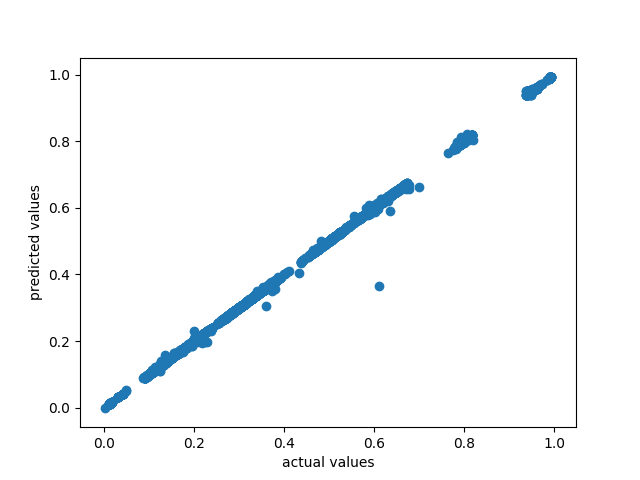
\includegraphics[width=0.5\textwidth]{LDH_D_PDH_dtr}
\caption[Decision Tree Regressor scatter plot of actual vs predict values for \string(LDH\textunderscore D, PDH) dial]
{Decision Tree Regressor scatter plot of actual vs predict values for \string(LDH\textunderscore D, PDH) dial\index{Decision Tree Regressor scatter plot for \string(LDH\textunderscore D, PDH) dial}}
\label{fig:LdhPdhDtr}
\end{figure}

%\vspace{-0.25in}
\begin{figure}[h] 
\centering
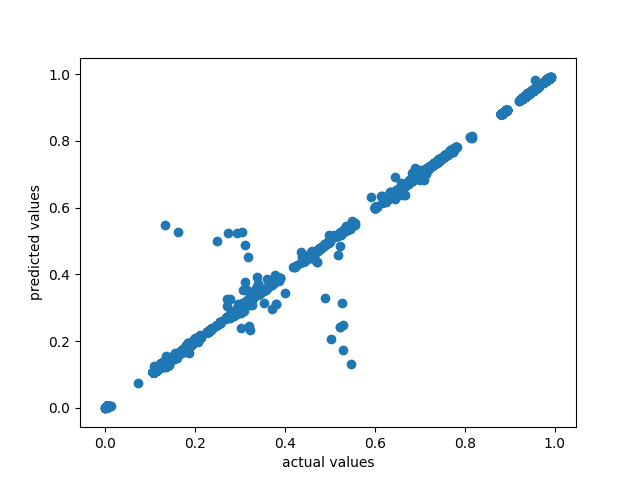
\includegraphics[width=0.5\textwidth]{PTAr_ACALD_dtr}
\caption[Decision Tree Regressor scatter plot of actual vs predict values for $(PTAr, ACALD)$ dial]
{Decision Tree Regressor scatter plot of actual vs predict values for $(PTAr, ACALD)$ dial\index{Decision Tree Regressor scatter plot for $(PTAr, ACALD)$ dial}}
\label{fig:PtarAcaldDtr}
\end{figure}

%\vspace{-0.25in}
\begin{figure}[h] 
\centering
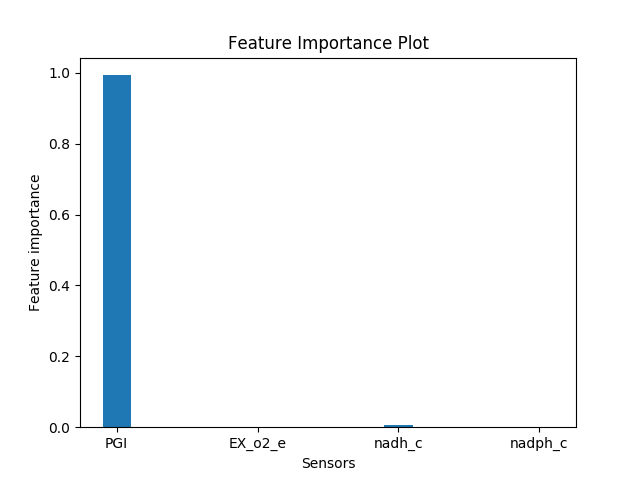
\includegraphics[width=0.5\textwidth]{PGI_G6PDH2r_dtr_important_features}
\caption[Decision Tree feature importance plot for $(PGI, G6PDH2r)$ dial]
{Decision Tree feature importance plot for $(PGI, G6PDH2r)$ dial\index{Feature importance plot for $(PGI, G6PDH2r)$ dial}}
\label{fig:PgiG6pdh2rDtrImp}
\end{figure}

%\vspace{-0.25in}
\begin{figure}[h] 
\centering
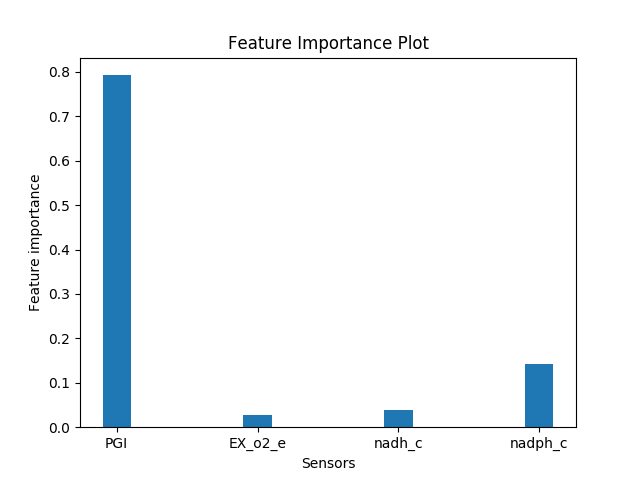
\includegraphics[width=0.5\textwidth]{PTAr_CS_dtr_important_features}
\caption[Decision Tree feature importance plot for $(PTAr, CS)$ dial]
{Decision Tree feature importance plot for $(PTAr, CS)$ dial\index{Feature importance plot for $(PTAr, CS)$ dial}}
\label{fig:PtarCsDtrImp}
\end{figure}

%\vspace{-0.25in}
\begin{figure}[h] 
\centering
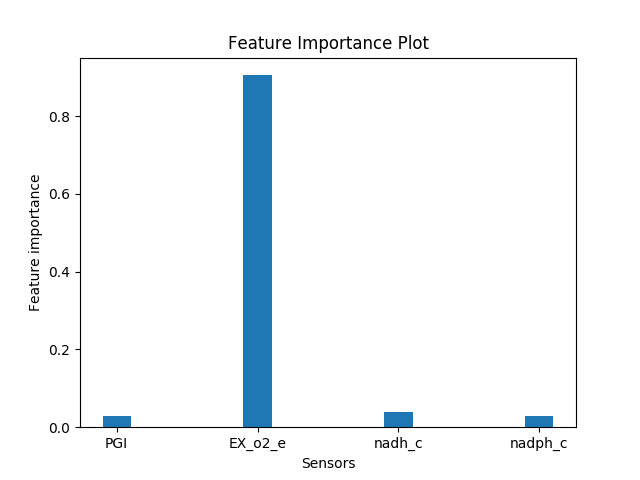
\includegraphics[width=0.5\textwidth]{PFL_PDH_dtr_important_features}
\caption[Decision Tree feature importance plot for $(PFL, PDH)$ dial]
{Decision Tree feature importance plot for $(PFL, PDH)$ dial\index{Feature importance plot for $(PFL, PDH)$ dial}}
\label{fig:PflPdhDtrImp}
\end{figure}

%\vspace{-0.25in}
\begin{figure}[h] 
\centering
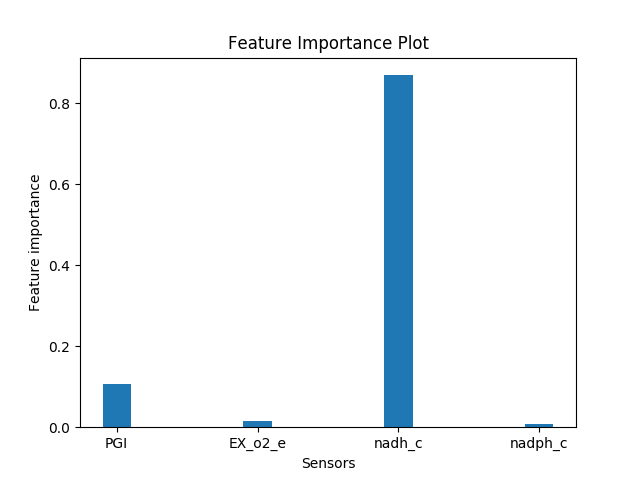
\includegraphics[width=0.5\textwidth]{LDH_D_PDH_dtr_important_features}
\caption[Decision Tree feature importance plot for \string(LDH\textunderscore D, PDH) dial]
{Decision Tree feature importance plot for \string(LDH\textunderscore D, PDH) dial\index{Feature importance plot for \string(LDH\textunderscore D, PDH) dial}}
\label{fig:LdhPdhDtrImp}
\end{figure}

%\vspace{-0.25in}
\begin{figure}[h] 
\centering
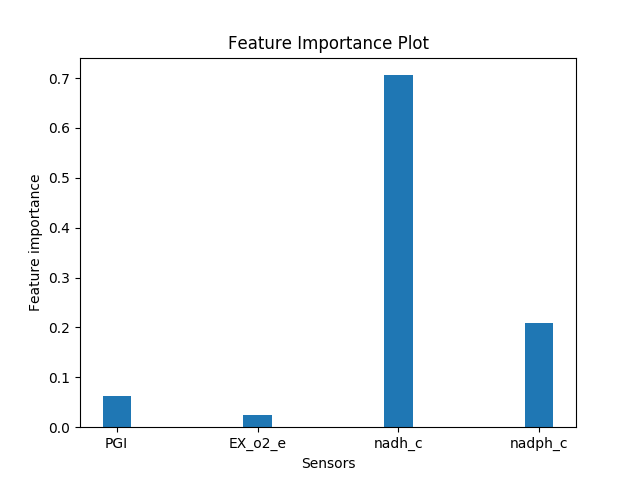
\includegraphics[width=0.5\textwidth]{PTAr_ACALD_dtr_important_features}
\caption[Decision Tree feature importance plot for $(PTAr, ACALD)$ dial]
{Decision Tree feature importance plot for $(PTAr, ACALD)$ dial\index{Feature importance plot for $(PTAr, ACALD)$ dial}}
\label{fig:PtarAcaldDtrImp}
\end{figure}
%%%%%%%%%%%%%%%%%%%%%%%%%%%%%%%%%%%%%%%%%%%%%%%%%%%%%%%%%%%%%%%%%%%%%%%%%%%%%%%%%%%

\section{Random Forest Regressor}\label{sec:rfrRes}
Table \ref{tab:Rfr} reflects the results from random forest regressor.
From figures \ref{fig:PgiG6pdh2rRfr}, \ref{fig:PtarCsRfr}, \ref{fig:PflPdhRfr}, \ref{fig:LdhPdhRfr} and \ref{fig:PtarAcaldRfr}, we can see that the random forest regressor performs marginally better than decision tree regressor. It's the closest to the actual value with precision up to 6 decimal places.
Figures \ref{fig:PgiG6pdh2rRfrImp}, \ref{fig:PtarCsRfrImp}, \ref{fig:PflPdhRfrImp}, \ref{fig:LdhPdhRfrImp} and \ref{fig:PtarAcaldRfrImp} shows the feature importance plots for each of the dials.\\
For \string(PGI, G6PDH2r) dial, from the figure \ref{fig:PgiG6pdh2rRfrImp}, it can be seen that PGI sensor is the dominating feature. Since statistical models depend largely on the dataset used to train them, it is obvious for PGI sensor to be the dominating feature since PGI is part of both input and output.\\ 

\vspace{0.25in}
\begin{table}[!ht]
\caption[Random Forest Regressor results]{Results from Random Forest Regressor}

\vspace{-0.25in}
\begin{center}
\begin{tabular}{|p{1.3in}|p{1in}|p{1in}|p{1.1in}|}
\hline
Dial & MSE  & Pearson-r & Coefficient R\string^2 \\

\hline
\string(PGI, G6PDH2r) & 1.92471e-06 & 0.999991 & 0.9999994 \\

\hline
\string(LDH\textunderscore D, PDH) & 3.11794e-07 & 0.999998 & 0.999995\\

\hline
\string(PFL, PDH) & 2.84958e-06 & 0.999987 & 0.999993\\

\hline
\string(PTAr, ACALD) &  1.33654e-05 & 0.999917 & 0.999974\\

\hline
\string(PTAr, CS) & 9.5527e-06 & 0.999950 & 0.999981\\

\hline

\end{tabular}
\end{center}
\label{tab:Rfr}
\end{table}

%\vspace{-0.25in}
\begin{figure}[h] 
\centering
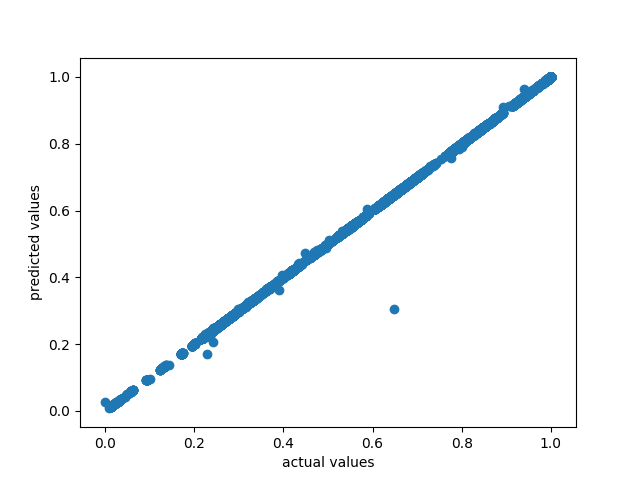
\includegraphics[width=0.5\textwidth]{PGI_G6PDH2r_rfr}
\caption[Random Forest Regressor scatter plot of actual vs predict values for $(PGI, G6PDH2r)$ dial]
{Random Forest Regressor scatter plot of actual vs predict values for $(PGI, G6PDH2r)$ dial\index{Random Forest Regressor scatter plot for $(PGI, G6PDH2r)$ dial}}
\label{fig:PgiG6pdh2rRfr}
\end{figure}

%\vspace{-0.25in}
\begin{figure}[h] 
\centering
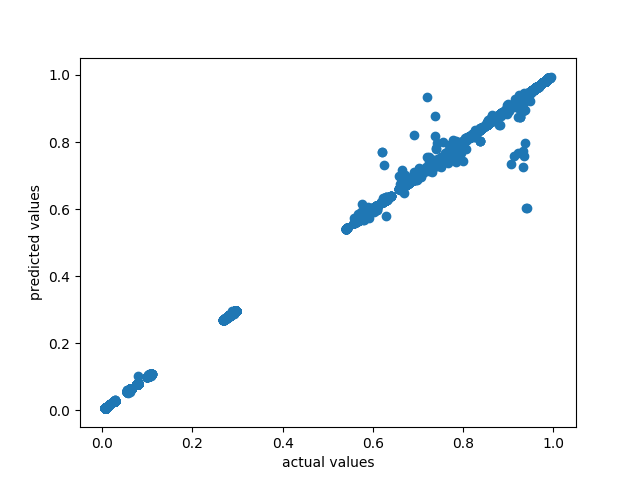
\includegraphics[width=0.5\textwidth]{PTAr_CS_rfr}
\caption[Random Forest Regressor scatter plot of actual vs predict values for $(PTAr, CS)$ dial]
{Random Forest Regressor scatter plot of actual vs predict values for $(PTAr, CS)$ dial\index{Random Forest Regressor scatter plot for $(PTAr, CS)$ dial}}
\label{fig:PtarCsRfr}
\end{figure}

%\vspace{-0.25in}
\begin{figure}[h] 
\centering
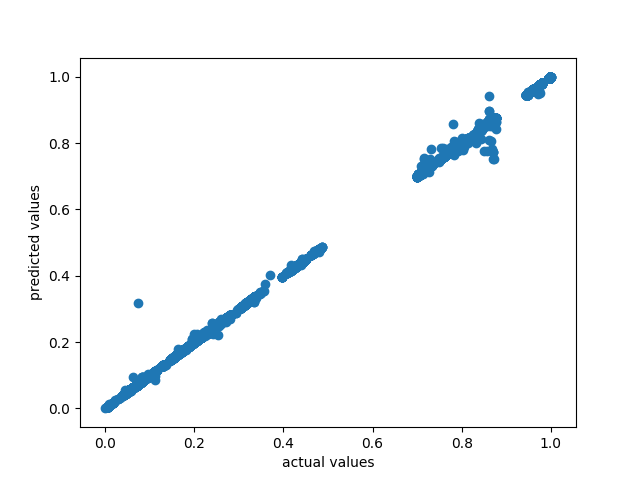
\includegraphics[width=0.5\textwidth]{PFL_PDH_rfr}
\caption[Random Forest Regressor scatter plot of actual vs predict values for $(PFL, PDH)$ dial]
{Random Forest Regressor scatter plot of actual vs predict values for $(PFL, PDH)$ dial\index{Random Forest Regressor scatter plot for $(PFL, PDH)$ dial}}
\label{fig:PflPdhRfr}
\end{figure}

%\vspace{-0.25in}
\begin{figure}[h] 
\centering
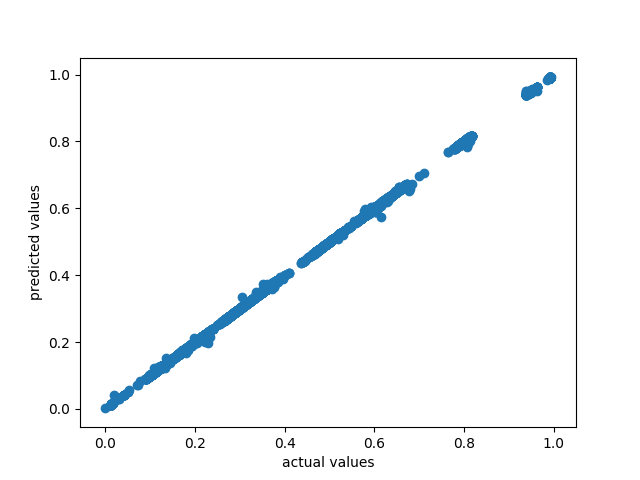
\includegraphics[width=0.5\textwidth]{LDH_D_PDH_rfr}
\caption[Random Forest scatter plot of actual vs predict values for \string(LDH\textunderscore D, PDH) dial]
{Random Forest Regressor scatter plot of actual vs predict values for $(LDH_D, PDH)$ dial\index{Random Forest Regressor scatter plot for \string(LDH\textunderscore D, PDH) dial}}
\label{fig:LdhPdhRfr}
\end{figure}

%\vspace{-0.25in}
\begin{figure}[h] 
\centering
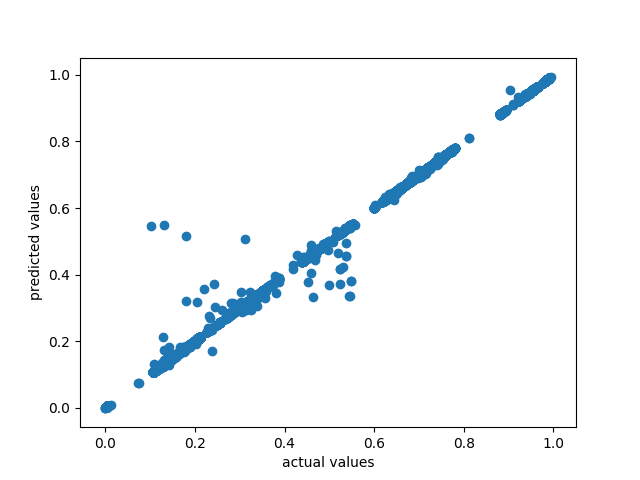
\includegraphics[width=0.5\textwidth]{PTAr_ACALD_rfr}
\caption[Random Forest Regressor scatter plot of actual vs predict values for $(PTAr, ACALD)$ dial]
{Random Forest Regressor scatter plot of actual vs predict values for $(PTAr, ACALD)$ dial\index{Random Forest Regressor scatter plot for $(PTAr, ACALD)$ dial}}
\label{fig:PtarAcaldRfr}
\end{figure}

%\vspace{-0.25in}
\begin{figure}[h] 
\centering
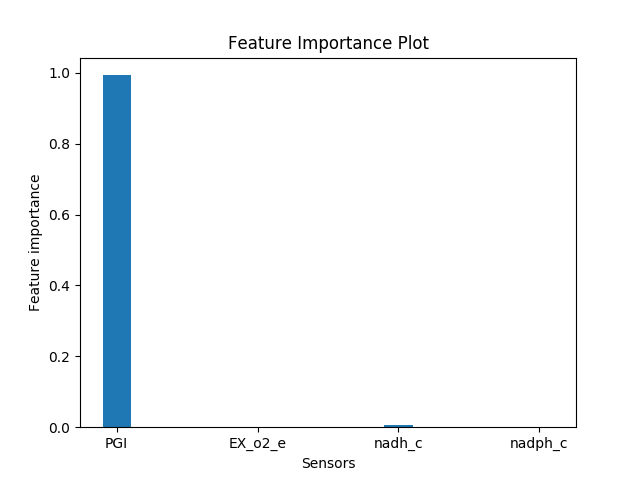
\includegraphics[width=0.5\textwidth]{PGI_G6PDH2r_rfr_important_features}
\caption[Random Forest feature importance plot for $(PGI, G6PDH2r)$ dial]
{Random Forest feature importance plot for $(PGI, G6PDH2r)$ dial\index{Feature importance plot for $(PGI, G6PDH2r)$ dial}}
\label{fig:PgiG6pdh2rRfrImp}
\end{figure}

%\vspace{-0.25in}
\begin{figure}[h] 
\centering
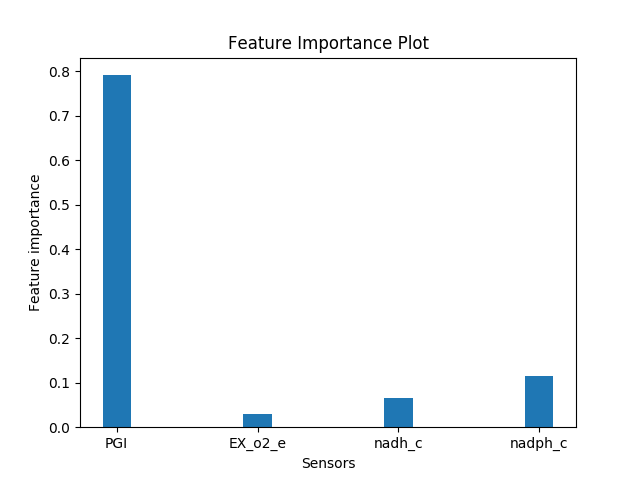
\includegraphics[width=0.5\textwidth]{PTAr_CS_rfr_important_features}
\caption[Random Forest feature importance plot for $(PTAr, CS)$ dial]
{Random Forest feature importance plot for $(PTAr, CS)$ dial\index{Feature importance plot for $(PTAr, CS)$ dial}}
\label{fig:PtarCsRfrImp}
\end{figure}

%\vspace{-0.25in}
\begin{figure}[h] 
\centering
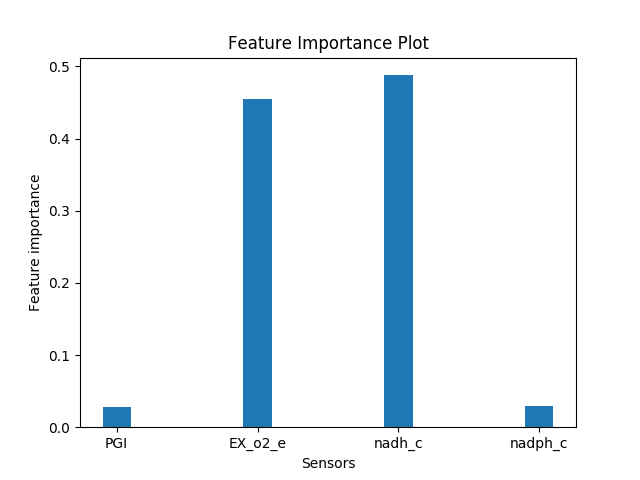
\includegraphics[width=0.5\textwidth]{PFL_PDH_rfr_important_features}
\caption[Random Forest feature importance plot for $(PFL, PDH)$ dial]
{Random Forest feature importance plot for $(PFL, PDH)$ dial\index{Feature importance plot for $(PFL, PDH)$ dial}}
\label{fig:PflPdhRfrImp}
\end{figure}

%\vspace{-0.25in}
\begin{figure}[h] 
\centering
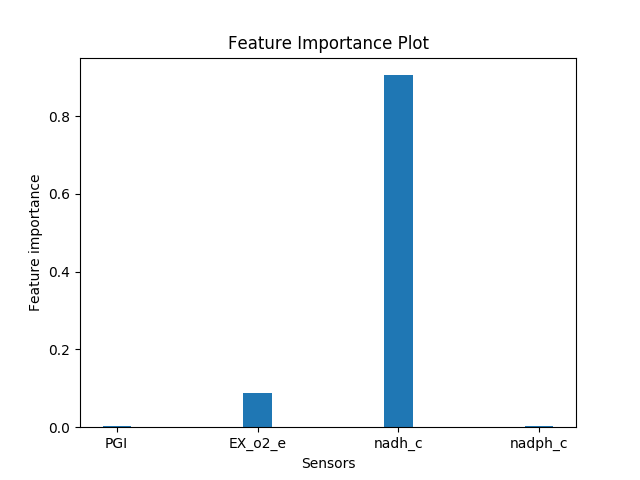
\includegraphics[width=0.5\textwidth]{LDH_D_PDH_rfr_important_features}
\caption[Random Forest feature importance plot for \string(LDH\textunderscore D, PDH) dial]
{Random Forest feature importance plot for \string(LDH\textunderscore D, PDH) dial\index{Feature importance plot for \string(LDH\textunderscore D, PDH) dial}}
\label{fig:LdhPdhRfrImp}
\end{figure}

%\vspace{-0.25in}
\begin{figure}[h] 
\centering
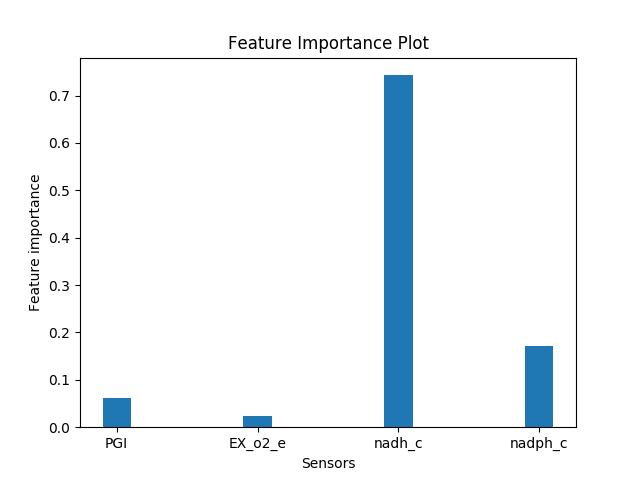
\includegraphics[width=0.5\textwidth]{PTAr_ACALD_rfr_important_features}
\caption[Random Forest feature importance plot for $(PTAr, ACALD)$ dial]
{Random Forest feature importance plot for $(PTAr, ACALD)$ dial\index{Feature importance plot for $(PTAr, ACALD)$ dial}}
\label{fig:PtarAcaldRfrImp}
\end{figure}

\textbf{biological significance of feature importance plots}
%%%%%%%%%%%%%%%%%%%%%%%%%%%%%%%%%%%%%%%%%%%%%%%%%%%%%%%%%%%%%%%%%%%%%%%%%%%%%%
%%%%%%%%%%%%%%%%%%%%%%%%%%%%%%%%%%%%%%%%%%%%%%%%%%%%%%%%%%%%%%%%%%%%%%%%%%%%%%
\chapter{Conclusion}
\textbf{TODO: Ask Zak about biological significance of feature importance plots}\\
Table \ref{tab:Results} presents a consolidation of results from all the statistical methods employed in this project. The average and standard deviation (stdev) values of MSE, Pearson-r and Coefficient $R\string^2$ are calculated for each method and are reported in table \ref{tab:Results}. From the table \ref{tab:Results}, it is evident that through statistical modeling, dial values can be predicted effectively using sensors. 
\vspace{0.25in}
\begin{table}[!ht]
\caption[Combined Results from All Methods]{Combined Results from All Methods}

\vspace{-0.25in}
\begin{center}
\begin{tabular}{|p{0.85in}|p{0.8in}|p{0.8in}|p{0.8in}|p{0.85in}|p{0.8in}|p{0.8in}|}
\hline
Method & Average MSE  & Stdev of MSE & Average Pearson-r & Stdev of Pearson-r & Average Coefficient R\string^2 & Stdev of Coefficient R\string^2\\

\hline
Linear Regression & 0.01784 & 0.007576 & 0.900479 & 0.054857 & 0.80518 & 0.093599 \\

\hline
Extreme Gradient Boosted Trees & 0.000811 & 0.000377 & 0.99670 & 0.00188 & 0.99149 & 0.004834\\

\hline
Decision Tree Regressor & 7.98279e-06 & 6.3735e-06 & 0.99995 & 4.01995e-05 & 0.99990 & 7.98498e-05\\

\hline
Random Forest Regressor &  5.6008e-06 & 4.9992e-06 & 0.999968 & 3.0702e-05 & 0.999988 & 9.46369e-06\\

\hline

\end{tabular}
\end{center}
\label{tab:Results}
\end{table}

%%%%%%%%%%%%%%%%%%%%%%%%%%%%%%%%%%%%%%%%%%%%%%%%%%%%%%%%%%%%%%%%%%%%%%%%%%%%%%
%%%%%%%%%%%%%%%%%%%%%%%%%%%%%%%%%%%%%%%%%%%%%%%%%%%%%%%%%%%%%%%%%%%%%%%%%%%%%%
\chapter{Future Work}
\textbf{TODO: Ask Zak about it}
%% END MATTER
%\printindex %% Uncomment to display the index
% \nocite{}  %% Put any references that you want to include in the bib 
%               but haven't cited in the braces.
\bibliographystyle{alpha}  %% This is just my personal favorite style. 
%                              There are many others.
%\setlength{\bibleftmargin}{0.25in}  % indent each item
%\setlength{\bibindent}{-\bibleftmargin}  % unindent the first line
\def\baselinestretch{1.0}  % force single spacing
%\setlength{\bibitemsep}{0.16in}  % add extra space between items
\bibliography{template}  %% This looks for the bibliography in template.bib 
%                          which should be formatted as a bibtex file.
%                          and needs to be separately compiled into a bbl file.
\end{document}

